\documentclass[12pt, a4paper]{book}

% =====================================================================
%  PACKAGES
% =====================================================================
\usepackage{amsmath}
\usepackage{amssymb}
\usepackage{amsthm}
\usepackage{mathtools}
\usepackage{tikz}
\usepackage{pgfplots}
\pgfplotsset{compat=1.18}
\usetikzlibrary{arrows.meta, calc, decorations.pathreplacing,
                decorations.markings, angles, quotes, patterns,
                decorations.pathreplacing}
\usepackage{tcolorbox}
\tcbuselibrary{skins, breakable, theorems}
\usepackage{physics}
\usepackage{enumitem}
\usepackage{booktabs}
\usepackage{geometry}
\usepackage{hyperref}
\usepackage{xcolor}
\usepackage{graphicx}
\usepackage{float}
\usepackage{multicol}
\usepackage{array}
\usepackage{cancel}
\usepackage{siunitx}
\usepackage{setspace}
\usepackage{fancyhdr}
\usepackage{titlesec}
\usepackage{microtype}

\geometry{
  a4paper,
  top=2.5cm, bottom=2.5cm,
  left=2.8cm, right=2.8cm,
  headheight=15pt
}

% =====================================================================
%  COLOURS
% =====================================================================
\definecolor{deepblue}{RGB}{10,50,120}
\definecolor{midblue}{RGB}{30,90,180}
\definecolor{lightblue}{RGB}{220,235,255}
\definecolor{tealgreen}{RGB}{0,110,100}
\definecolor{lightgreen}{RGB}{220,245,235}
\definecolor{warmred}{RGB}{180,30,30}
\definecolor{lightyellow}{RGB}{255,252,220}
\definecolor{lightorange}{RGB}{255,235,210}
\definecolor{lightpurple}{RGB}{240,225,255}
\definecolor{darkgray}{RGB}{60,60,60}
\definecolor{medgray}{RGB}{120,120,120}

% =====================================================================
%  THEOREM ENVIRONMENTS
% =====================================================================
\tcbuselibrary{most}

\newtcbtheorem[number within=section]{defn}{Definition}{
  enhanced, breakable,
  colback=lightblue, colframe=deepblue, colbacktitle=deepblue,
  fonttitle=\bfseries\sffamily, coltitle=white,
  attach boxed title to top left={yshift=-2mm, xshift=4mm},
  boxed title style={colframe=deepblue},
  separator sign={.\ },
}{def}

\newtcbtheorem[number within=section]{thm}{Theorem}{
  enhanced, breakable,
  colback=lightgreen, colframe=tealgreen, colbacktitle=tealgreen,
  fonttitle=\bfseries\sffamily, coltitle=white,
  attach boxed title to top left={yshift=-2mm, xshift=4mm},
  boxed title style={colframe=tealgreen},
  separator sign={.\ },
}{thm}

\newtcbtheorem[number within=section]{prop}{Proposition}{
  enhanced, breakable,
  colback=lightgreen!60, colframe=tealgreen!80, colbacktitle=tealgreen!80,
  fonttitle=\bfseries\sffamily, coltitle=white,
  attach boxed title to top left={yshift=-2mm, xshift=4mm},
  separator sign={.\ },
}{prop}

\newtcbtheorem[number within=section]{cor}{Corollary}{
  enhanced, breakable,
  colback=lightgreen!40, colframe=tealgreen!60, colbacktitle=tealgreen!60,
  fonttitle=\bfseries\sffamily, coltitle=white,
  attach boxed title to top left={yshift=-2mm, xshift=4mm},
  separator sign={.\ },
}{cor}

\newtcbtheorem[number within=section]{exmp}{Example}{
  enhanced, breakable,
  colback=white, colframe=midblue, colbacktitle=midblue,
  fonttitle=\bfseries\sffamily, coltitle=white,
  attach boxed title to top left={yshift=-2mm, xshift=4mm},
  separator sign={.\ },
}{ex}

\newtcbtheorem[number within=section]{rmk}{Remark}{
  enhanced, breakable,
  colback=lightyellow, colframe=orange!70!black, colbacktitle=orange!70!black,
  fonttitle=\bfseries\sffamily, coltitle=white,
  attach boxed title to top left={yshift=-2mm, xshift=4mm},
  separator sign={.\ },
}{rmk}

% =====================================================================
%  SPECIAL BOXES
% =====================================================================
\newtcolorbox{intuition}[1][]{
  enhanced, breakable,
  title={\faLightbulb\quad Intuition},
  colback=lightyellow, colframe=orange!80!black, colbacktitle=orange!80!black,
  fonttitle=\bfseries\sffamily, coltitle=white,
  attach boxed title to top left={yshift=-2mm, xshift=4mm},
  #1
}

\newtcolorbox{intuitionbox}[1][Intuition]{
  enhanced, breakable,
  title={#1},
  colback=lightyellow, colframe=orange!70!black, colbacktitle=orange!70!black,
  fonttitle=\bfseries\sffamily\large, coltitle=white,
  boxrule=1pt,
  left=6pt, right=6pt, top=6pt, bottom=6pt,
}

\newtcolorbox{warningbox}[1][Warning]{
  enhanced, breakable,
  title={#1},
  colback=red!8, colframe=warmred, colbacktitle=warmred,
  fonttitle=\bfseries\sffamily\large, coltitle=white,
  boxrule=1pt,
  left=6pt, right=6pt, top=6pt, bottom=6pt,
}

\newtcolorbox{explorationbox}[1][Exploration]{
  enhanced, breakable,
  title={#1},
  colback=lightpurple, colframe=purple!60!black, colbacktitle=purple!60!black,
  fonttitle=\bfseries\sffamily\large, coltitle=white,
  boxrule=1pt,
  left=6pt, right=6pt, top=6pt, bottom=6pt,
}

\newtcolorbox{historicalbox}[1][Historical Note]{
  enhanced, breakable,
  title={#1},
  colback=brown!8, colframe=brown!60!black, colbacktitle=brown!60!black,
  fonttitle=\bfseries\sffamily\large, coltitle=white,
  boxrule=1pt,
  left=6pt, right=6pt, top=6pt, bottom=6pt,
}

\newtcolorbox{examtrap}[1][Exam Trap]{
  enhanced, breakable,
  title={#1},
  colback=orange!10, colframe=orange!80!black, colbacktitle=orange!80!black,
  fonttitle=\bfseries\sffamily\large, coltitle=white,
  boxrule=1pt,
  left=6pt, right=6pt, top=6pt, bottom=6pt,
}

\newtcolorbox{summarybox}[1][Chapter Summary]{
  enhanced, breakable,
  title={#1},
  colback=lightblue, colframe=deepblue, colbacktitle=deepblue,
  fonttitle=\bfseries\sffamily\large, coltitle=white,
  boxrule=1.5pt,
  left=8pt, right=8pt, top=8pt, bottom=8pt,
}

% =====================================================================
%  PAGE STYLE
% =====================================================================
\pagestyle{fancy}
\fancyhf{}
\fancyhead[LE]{\small\sffamily\color{medgray}\leftmark}
\fancyhead[RO]{\small\sffamily\color{medgray}\rightmark}
\fancyfoot[C]{\small\sffamily\color{medgray}\thepage}
\renewcommand{\headrulewidth}{0.4pt}

\titleformat{\chapter}[display]
  {\normalfont\huge\bfseries\sffamily\color{deepblue}}
  {\normalfont\Large\sffamily\color{midblue}Chapter \thechapter}{12pt}{\Huge}
\titleformat{\section}{\large\bfseries\sffamily\color{deepblue}}{\thesection}{1em}{}
\titleformat{\subsection}{\normalsize\bfseries\sffamily\color{midblue}}{\thesubsection}{1em}{}

% =====================================================================
%  CUSTOM COMMANDS
% =====================================================================
\newcommand{\vect}[1]{\mathbf{#1}}
\newcommand{\uvec}[1]{\hat{\mathbf{#1}}}
\newcommand{\R}{\mathbb{R}}
\newcommand{\ii}{\mathbf{i}}
\newcommand{\jj}{\mathbf{j}}
\newcommand{\kk}{\mathbf{k}}
\newcommand{\Fvec}{\mathbf{F}}
\newcommand{\rvec}{\mathbf{r}}
\newcommand{\vvec}{\mathbf{v}}
\newcommand{\avec}{\mathbf{a}}
\newcommand{\half}{\tfrac{1}{2}}
\newcommand{\ms}{\,\mathrm{ms}^{-1}}
\newcommand{\mss}{\,\mathrm{ms}^{-2}}
\newcommand{\Nm}{\,\mathrm{Nm}}
\newcommand{\kg}{\,\mathrm{kg}}
\newcommand{\m}{\,\mathrm{m}}
\newcommand{\N}{\,\mathrm{N}}
\newcommand{\rad}{\,\mathrm{rad}}
\newcommand{\rads}{\,\mathrm{rad\,s}^{-1}}

% =====================================================================
%  DOCUMENT
% =====================================================================
\begin{document}

\frontmatter

% ----- Title Page -----
\begin{titlepage}
\centering
\vspace*{2cm}
{\color{deepblue}\rule{\textwidth}{2pt}}\\[0.5cm]
{\Huge\bfseries\sffamily\color{deepblue} Further Mechanics}\\[0.3cm]
{\Large\sffamily\color{midblue} University-Preparation Notes}\\[0.2cm]
{\color{deepblue}\rule{\textwidth}{2pt}}\\[1.5cm]

\begin{tcolorbox}[colback=lightblue, colframe=deepblue, width=0.85\textwidth]
\centering
{\large\sffamily Covering:}\\[0.4cm]
\begin{tabular}{ll}
\textbf{Chapter 13} & Projectiles \\[4pt]
\textbf{Chapter 14} & Equilibrium of a Rigid Body \\[4pt]
\textbf{Chapter 15} & Circular Motion \\[4pt]
\textbf{Chapter 16} & Hooke's Law \\[4pt]
\textbf{Chapter 17} & Linear Motion Under a Variable Force \\[4pt]
\textbf{Chapter 18} & Momentum \\
\end{tabular}
\end{tcolorbox}

\vspace{1.5cm}
{\large\sffamily\color{darkgray} For the Ambitious A-Level Further Mathematics Student}\\[0.3cm]
{\normalsize\sffamily\color{medgray} Targeting Oxford, Cambridge, Imperial, Warwick, MIT and similar}
\vfill
{\large\sffamily\bfseries Author: Rayyan Hanif Kolej MARA Seremban}\\[0.3cm]
{\normalsize\sffamily\color{medgray} A-Level Further Mathematics}
\vspace{1cm}
{\color{deepblue}\rule{\textwidth}{1pt}}
\end{titlepage}

% ----- Preface -----
\chapter*{Preface}
\addcontentsline{toc}{chapter}{Preface}

These notes are written for the student who is not content with merely passing examinations --- the student who wants to \emph{understand} mechanics deeply, to see where every formula comes from, to feel why each result is true before it is proved, and to glimpse the vast landscape of physics and mathematics that lies beyond the A-Level syllabus.

The six chapters here cover the Further Mechanics content of A-Level Further Mathematics. However, the treatment goes considerably beyond what is needed for examinations. You will find:

\begin{itemize}[leftmargin=2em]
  \item Every major result derived carefully from first principles.
  \item Physical and geometric intuition built before formulas are introduced.
  \item Connections to university mathematics (variational mechanics, rigid body dynamics, Hamiltonian mechanics, wave mechanics).
  \item Historical notes placing each discovery in context.
  \item Challenging extension questions designed to stretch even the strongest students.
\end{itemize}

\noindent\textbf{How to use these notes.} Read each introduction carefully. Before looking at a derivation, try to predict the answer. After a worked example, close the notes and attempt it yourself. Engage with the Exploration boxes --- these contain the deepest material.

\vspace{1cm}
\noindent\textit{Rayyan Hanif AL25.1}

\tableofcontents

\mainmatter

% =====================================================================
% =====================================================================
%  CHAPTER 13: PROJECTILES
% =====================================================================
% =====================================================================
\chapter{Projectiles}

\section{Introduction}

\subsection{What is Projectile Motion?}

When an object is launched into the air and then moves freely under gravity alone --- with no thrust, no air resistance, no string --- we call it a \textbf{projectile}, and we call its motion \textbf{projectile motion}.

\begin{intuitionbox}
Think of a football kicked at an angle, a ball thrown across a room, or a stone hurled from a cliff. In all these cases, after the initial impulse, the only force acting is gravity, which pulls straight down. This beautifully simple situation turns out to have an elegant mathematical structure.
\end{intuitionbox}

Why is this important? Projectile motion is the simplest example of \emph{two-dimensional kinematics}. It shows us how to decompose a problem into independent components, a strategy that appears throughout all of mechanics and physics. It also introduces the concept of a trajectory --- the curve traced by the particle --- and we will derive that this curve is always a parabola, one of the classical conic sections.

\subsection{Why the Independence of Components Works}

The key physical insight is Newton's Second Law: $\Fvec = m\avec$. The gravitational force acts only vertically:
\[
  \Fvec = \begin{pmatrix}0 \\ -mg\end{pmatrix}
\]
so the acceleration is $\avec = \begin{pmatrix}0 \\ -g\end{pmatrix}$. 

Since horizontal acceleration is zero and vertical acceleration is $-g$, the horizontal and vertical motions are \emph{completely independent}. We can analyse them separately and then combine the results.

\begin{historicalbox}
Galileo Galilei (1564--1642) was the first to understand projectile motion correctly. Before Galileo, it was believed that a projectile moved horizontally until it ``ran out of impetus'', then fell vertically. Galileo's genius was to see that horizontal and vertical motions are independent, and that the trajectory is parabolic. He described this in his \textit{Discourses and Mathematical Demonstrations Relating to Two New Sciences} (1638), one of the founding documents of modern physics.
\end{historicalbox}

\section{Motion in the Vertical Plane}

\subsection{Setting Up the Problem}

\begin{defn}{Coordinate System for Projectiles}{}
We place the origin at the initial position of the particle. The $x$-axis is horizontal (in the direction of initial horizontal motion) and the $y$-axis is vertical (upward positive). Time $t$ is measured from the moment of projection.
\end{defn}

A particle is projected with initial speed $u$ at angle $\alpha$ above the horizontal.

\begin{center}
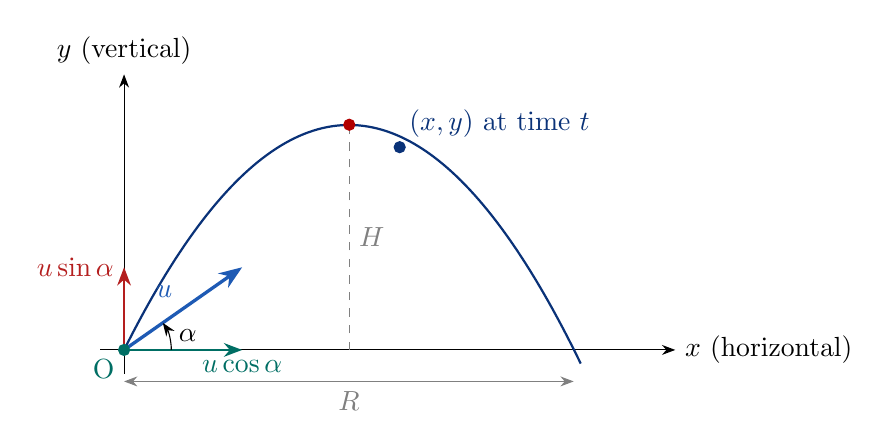
\begin{tikzpicture}[scale=1.0, >=Stealth]
  % Axes
  \draw[->] (-0.3,0) -- (7,0) node[right] {$x$ (horizontal)};
  \draw[->] (0,-0.3) -- (0,3.5) node[above] {$y$ (vertical)};
  
  % Trajectory (parabola)
  \draw[thick, deepblue, domain=0:5.8, samples=100]
    plot (\x, {2*\x - 0.35*\x*\x});
  
  % Initial velocity vector
  \draw[->, very thick, midblue] (0,0) -- (1.5, 1.05) node[midway, above left] {$u$};
  
  % Components
  \draw[->, thick, tealgreen] (0,0) -- (1.5, 0) node[below] {$u\cos\alpha$};
  \draw[->, thick, warmred] (0,0) -- (0, 1.05) node[left] {$u\sin\alpha$};
  
  % Angle arc
  \draw[->] (0.6,0) arc (0:35:0.6) node[midway, right] {$\alpha$};
  
  % Point on trajectory
  \filldraw[deepblue] (3.5, 2.575) circle (2pt) node[above right] {$(x,y)$ at time $t$};
  
  % Maximum height label
  \draw[dashed, gray] (2.86, 0) -- (2.86, 2.86) node[midway, right] {$H$};
  \filldraw[red!70!black] (2.86, 2.86) circle (2pt);
  
  % Range label
  \draw[<->, gray] (0, -0.4) -- (5.71, -0.4) node[midway, below] {$R$};
  \filldraw[tealgreen] (0,0) circle (2pt) node[below left] {O};
\end{tikzpicture}
\end{center}

\subsection{Deriving the Equations of Motion}

Starting from Newton's Second Law:
\[
  \ddot{x} = 0, \qquad \ddot{y} = -g
\]

\textbf{Horizontal:} Integrating $\ddot{x} = 0$ twice with initial conditions $\dot{x}(0) = u\cos\alpha$, $x(0) = 0$:
\[
  \dot{x} = u\cos\alpha, \qquad x = ut\cos\alpha
\]

\textbf{Vertical:} Integrating $\ddot{y} = -g$ twice with initial conditions $\dot{y}(0) = u\sin\alpha$, $y(0) = 0$:
\[
  \dot{y} = u\sin\alpha - gt, \qquad y = ut\sin\alpha - \frac{1}{2}gt^2
\]

\begin{thm}{Equations of Projectile Motion}{}
For a particle projected from the origin with speed $u$ at angle $\alpha$ above the horizontal:
\begin{align}
  x &= ut\cos\alpha \label{eq:proj_x}\\
  y &= ut\sin\alpha - \tfrac{1}{2}gt^2 \label{eq:proj_y}\\
  \dot{x} &= u\cos\alpha \label{eq:proj_vx}\\
  \dot{y} &= u\sin\alpha - gt \label{eq:proj_vy}
\end{align}
\end{thm}

\subsection{Time of Flight, Range, and Maximum Height}

\begin{thm}{Key Results for Projectile on Level Ground}{}
Assuming the particle lands at $y = 0$ (same height as projection):

\medskip
\textbf{Time of flight:} Set $y = 0$:
\[
  ut\sin\alpha - \tfrac{1}{2}gt^2 = 0 \implies t(u\sin\alpha - \tfrac{1}{2}gt) = 0
\]
Discarding $t = 0$:
\[
  \boxed{T = \frac{2u\sin\alpha}{g}}
\]

\textbf{Range:} $R = uT\cos\alpha$:
\[
  \boxed{R = \frac{u^2\sin 2\alpha}{g}}
\]

\textbf{Maximum height:} At maximum height $\dot{y} = 0$, so $t_{\max} = \tfrac{u\sin\alpha}{g}$:
\[
  \boxed{H = \frac{u^2\sin^2\alpha}{2g}}
\]
\end{thm}

\begin{intuitionbox}
\textbf{Maximum range at $\alpha = 45^\circ$:} Since $R = \frac{u^2\sin 2\alpha}{g}$, and $\sin 2\alpha$ is maximised when $2\alpha = 90^\circ$, i.e., $\alpha = 45^\circ$. This is the ``optimal angle'' result, familiar from sport. 

Notice the beautiful symmetry: ranges are equal for $\alpha$ and $(90^\circ - \alpha)$, since $\sin(2\alpha) = \sin(180^\circ - 2\alpha)$.
\end{intuitionbox}

\begin{exmp}{Standard Projectile Problem}{}
A particle is projected from a point on level ground with speed $20\ms$ at $30^\circ$ to the horizontal. Find: (a) the time of flight, (b) the range, (c) the maximum height.

\medskip
\textbf{Solution.} Here $u = 20$, $\alpha = 30^\circ$, $g = 9.8\mss$.

(a) $T = \dfrac{2 \times 20 \times \sin 30^\circ}{9.8} = \dfrac{2 \times 20 \times 0.5}{9.8} = \dfrac{20}{9.8} \approx 2.04\,\mathrm{s}$

(b) $R = \dfrac{20^2 \sin 60^\circ}{9.8} = \dfrac{400 \times \frac{\sqrt{3}}{2}}{9.8} = \dfrac{200\sqrt{3}}{9.8} \approx 35.3\,\mathrm{m}$

(c) $H = \dfrac{20^2 \sin^2 30^\circ}{2 \times 9.8} = \dfrac{400 \times 0.25}{19.6} = \dfrac{100}{19.6} \approx 5.10\,\mathrm{m}$
\end{exmp}

\begin{exmp}{Particle Projected from a Height}{}
A ball is thrown horizontally at $15\ms$ from the edge of a cliff $45\m$ high. Find when and where it hits the ground.

\medskip
\textbf{Solution.} Here $\alpha = 0°$, so initial vertical velocity is zero.

Taking downward as positive $y$ from the cliff top:
\[
  y = \tfrac{1}{2}gt^2 \implies 45 = \tfrac{1}{2}(9.8)t^2 \implies t^2 = \frac{90}{9.8} \implies t = 3.03\,\mathrm{s}
\]
Horizontal distance: $x = 15 \times 3.03 = 45.5\,\mathrm{m}$ from the base of the cliff.
\end{exmp}

\section{The Cartesian Equation of the Trajectory}

\subsection{Eliminating $t$}

The parametric equations contain time $t$ as a parameter. To find the \emph{trajectory} --- the curve in the $xy$-plane --- we eliminate $t$.

From $x = ut\cos\alpha$:
\[
  t = \frac{x}{u\cos\alpha}
\]

Substituting into $y = ut\sin\alpha - \frac{1}{2}gt^2$:
\[
  y = u \cdot \frac{x}{u\cos\alpha} \cdot \sin\alpha - \frac{1}{2}g\left(\frac{x}{u\cos\alpha}\right)^2
\]

\begin{thm}{Cartesian Equation of the Trajectory}{}
\[
  \boxed{y = x\tan\alpha - \frac{gx^2}{2u^2\cos^2\alpha}}
\]
This can also be written using $\sec^2\alpha = 1 + \tan^2\alpha$:
\[
  y = x\tan\alpha - \frac{gx^2(1+\tan^2\alpha)}{2u^2}
\]
\end{thm}

\begin{thm}{The Trajectory is a Parabola}{}
Rewriting: $y = x\tan\alpha - \frac{g}{2u^2\cos^2\alpha}x^2$.

This is a quadratic in $x$: $y = Ax + Bx^2$ where $A = \tan\alpha > 0$ (for $0 < \alpha < 90^\circ$) and $B = -\dfrac{g}{2u^2\cos^2\alpha} < 0$.

Any equation of the form $y = Ax + Bx^2$ (with $B \neq 0$) defines a \textbf{parabola}. Completing the square confirms this. Therefore, \emph{all projectile trajectories are parabolic}.
\end{thm}

\begin{historicalbox}
The parabolic nature of trajectories was known to Galileo (1638) but had been recognised geometrically even earlier. The precise mathematical derivation using calculus became possible after Newton and Leibniz independently invented the calculus in the late 17th century.
\end{historicalbox}

\subsection{Finding $\alpha$ Given Range and Speed}

Given $u$ and $R$, we can find $\alpha$. Setting $y = 0$:
\[
  0 = x\tan\alpha - \frac{gx^2}{2u^2\cos^2\alpha} \implies R = \frac{u^2 \sin 2\alpha}{g}
\]
So:
\[
  \sin 2\alpha = \frac{gR}{u^2}
\]
This has two solutions: $2\alpha = \theta$ or $2\alpha = 180^\circ - \theta$, corresponding to the \textbf{two possible projection angles} for a given range (one below $45^\circ$, one above).

\begin{exmp}{Two Angles for the Same Range}{}
A particle is projected with speed $28\ms$. Find the angles at which it must be projected to hit a target $56\m$ away on level ground (take $g = 9.8$).

\medskip
\textbf{Solution.}
\[
  \sin 2\alpha = \frac{9.8 \times 56}{28^2} = \frac{548.8}{784} = 0.7
\]
\[
  2\alpha = \arcsin(0.7) = 44.4^\circ\quad\text{or}\quad 2\alpha = 180^\circ - 44.4^\circ = 135.6^\circ
\]
\[
  \alpha = 22.2^\circ\quad\text{or}\quad\alpha = 67.8^\circ
\]
Both angles give the same range. The $22.2^\circ$ trajectory is faster but lower; the $67.8^\circ$ trajectory is slower but higher.
\end{exmp}

\begin{exmp}{Challenging --- Projectile Over a Wall}{}
A particle is projected from a point $O$ with speed $u$ at angle $\alpha$. A wall of height $h$ stands at horizontal distance $d$ from $O$. Find the condition on $\alpha$ for the particle to clear the wall.

\medskip
\textbf{Solution.} At $x = d$, we require $y \geq h$:
\[
  d\tan\alpha - \frac{gd^2}{2u^2\cos^2\alpha} \geq h
\]
\[
  d\tan\alpha - \frac{gd^2(1+\tan^2\alpha)}{2u^2} \geq h
\]
Let $T = \tan\alpha$. This becomes:
\[
  dT - \frac{gd^2}{2u^2}(1 + T^2) \geq h
\]
\[
  \frac{gd^2}{2u^2}T^2 - dT + \left(h + \frac{gd^2}{2u^2}\right) \leq 0
\]
This is a quadratic inequality in $T = \tan\alpha$. The valid range of $\alpha$ corresponds to the interval between the roots (when the discriminant is non-negative).

Discriminant $\geq 0$:
\[
  d^2 - 4\cdot\frac{gd^2}{2u^2}\cdot\left(h + \frac{gd^2}{2u^2}\right) \geq 0
  \implies u^2 \geq gh + \frac{g^2d^2}{2u^2}
  \implies u^4 - 2ghu^2 - g^2d^2 \geq 0
\]
This gives the minimum launch speed to clear the wall at all.
\end{exmp}

\section{Common Mistakes in Projectile Problems}

\begin{warningbox}
\textbf{Common Mistake 1: Sign errors.}
Always define your coordinate system and sign convention \emph{at the start}. If upward is positive, then $g = +9.8\mss$ acts \emph{downward}, so the vertical equation of motion is $\ddot{y} = -g$. Mixing signs mid-solution is the most common source of error.
\end{warningbox}

\begin{warningbox}
\textbf{Common Mistake 2: Using $y = ut - \frac{1}{2}gt^2$ when projected from a height.}
This equation is only valid when the particle starts at the origin. If the particle starts at height $H$, you must use $y = H + ut\sin\alpha - \frac{1}{2}gt^2$, or reset coordinates so the initial position is the origin.
\end{warningbox}

\begin{warningbox}
\textbf{Common Mistake 3: Forgetting that time is the same in both components.}
Both $x$ and $y$ are functions of the \emph{same} $t$. Students sometimes find $t$ from the horizontal equation and forget to check consistency with the vertical, or vice versa.
\end{warningbox}

\begin{examtrap}
\textbf{Exam Trap: $g = 9.8$ vs $g = 10$.}
Unless the problem specifies, use $g = 9.8\mss$. Some questions explicitly state to use $g = 10\mss$ for simplicity. Misreading this can cost marks even if your method is correct.
\end{examtrap}

\section{Advanced Exploration}

\subsection{Projectile on an Inclined Plane}

Suppose the ground is inclined at angle $\beta$ to the horizontal and the particle is projected at angle $\alpha$ \emph{above the incline} with speed $u$.

\begin{explorationbox}
It is elegant to resolve along and perpendicular to the incline. Let $x'$ be along the incline (up positive) and $y'$ be perpendicular (away from the incline). Then:
\begin{align*}
  \ddot{x'} &= -g\sin\beta, \qquad \dot{x'}(0) = u\cos\alpha, \qquad x'(0) = 0 \\
  \ddot{y'} &= -g\cos\beta, \qquad \dot{y'}(0) = u\sin\alpha, \qquad y'(0) = 0
\end{align*}

The particle hits the incline when $y' = 0$:
\[
  t = \frac{2u\sin\alpha}{g\cos\beta}
\]

Range along the incline:
\[
  R = x'(t) = \frac{u^2}{g\cos^2\beta}\left[2\sin\alpha\cos(\alpha+\beta)\right] = \frac{u^2}{g\cos^2\beta}\sin(2\alpha+\beta)\cos\beta - \ldots
\]

The maximum range is achieved at $\alpha = \frac{\pi}{4} - \frac{\beta}{2}$, i.e., when the direction of projection bisects the angle between the incline and the vertical. This is a beautiful result.
\end{explorationbox}

\subsection{Envelope of Trajectories}

For a fixed initial speed $u$, different angles $\alpha$ give different parabolic trajectories. The set of all such trajectories has an \textbf{envelope} --- a curve tangent to every trajectory. Points outside this envelope cannot be reached by any trajectory with speed $u$.

\begin{explorationbox}
From the trajectory equation $y = x\tan\alpha - \frac{g(1+\tan^2\alpha)}{2u^2}x^2$, setting $\frac{\partial}{\partial\alpha}(\ldots) = 0$ and eliminating $\alpha$:

\[
  y = \frac{u^2}{2g} - \frac{g}{2u^2}x^2
\]

This is itself a parabola! It is called the \textbf{parabola of safety}. Points inside this parabola (below and close to the origin) can be reached; points above it cannot. This has military applications (the range of a cannon) and sports applications (the maximum reach of a tennis serve).
\end{explorationbox}

\section{Connections}

\begin{itemize}[leftmargin=2em]
  \item \textbf{SUVAT equations}: Projectile motion uses the standard SUVAT equations in each component separately.
  \item \textbf{Vectors}: The velocity at any time is $\vvec = (u\cos\alpha)\,\ii + (u\sin\alpha - gt)\,\jj$.
  \item \textbf{Conic sections (Pure Maths)}: The trajectory is a parabola, which students will study in Further Pure.
  \item \textbf{Differential equations}: The equations $\ddot{x} = 0$, $\ddot{y} = -g$ are the simplest second-order ODEs --- constant acceleration.
  \item \textbf{University}: In fluid mechanics and aerodynamics, air resistance is added, making the equations nonlinear and requiring numerical methods.
\end{itemize}

\begin{summarybox}[Chapter 13 Summary: Projectiles]
\begin{itemize}[leftmargin=1.5em]
  \item Horizontal: $x = ut\cos\alpha$, $\dot{x} = u\cos\alpha$ (constant velocity)
  \item Vertical: $y = ut\sin\alpha - \frac{1}{2}gt^2$, $\dot{y} = u\sin\alpha - gt$
  \item Time of flight: $T = \frac{2u\sin\alpha}{g}$
  \item Range: $R = \frac{u^2\sin 2\alpha}{g}$; maximum at $\alpha = 45^\circ$
  \item Maximum height: $H = \frac{u^2\sin^2\alpha}{2g}$
  \item Trajectory: $y = x\tan\alpha - \frac{gx^2\sec^2\alpha}{2u^2}$ (a parabola)
  \item Two angles give the same range; they sum to $90^\circ$
\end{itemize}
\end{summarybox}

% =====================================================================
% =====================================================================
%  CHAPTER 14: EQUILIBRIUM OF A RIGID BODY
% =====================================================================
% =====================================================================
\chapter{Equilibrium of a Rigid Body}

\section{Introduction}

\subsection{From Particles to Rigid Bodies}

So far in mechanics, we have mostly treated objects as \emph{particles} --- mathematical points with mass but no size. Real objects, however, have extent. A ladder leaning against a wall, a beam supported at its ends, a hanging sign --- these are \emph{rigid bodies}: objects whose shape does not change under the forces applied.

For a rigid body, we must consider not just whether the net force is zero (which would prevent linear acceleration) but also whether the net \emph{turning effect} is zero (which would prevent rotation). This turns a simple question into something richer and more interesting.

\begin{intuitionbox}
Think about opening a door. Pushing near the hinge does very little; pushing near the edge moves it easily. The \emph{position} of the force matters, not just its magnitude. This turning effect is called the \textbf{moment} of the force, and it is the central concept of this chapter.
\end{intuitionbox}

\section{The Moment of a Force}

\subsection{Definition and Intuition}

\begin{defn}{Moment of a Force}{}
The \textbf{moment} of a force $F$ about a point $P$ is defined as:
\[
  M = F \times d
\]
where $d$ is the \textbf{perpendicular distance} from $P$ to the \emph{line of action} of $F$.

The SI unit of moment is the \textbf{newton-metre} ($\mathrm{N\,m}$).

Moments are \textbf{signed}: conventionally, anticlockwise moments are positive and clockwise moments are negative (though the choice is arbitrary as long as it is consistent).
\end{defn}

\begin{center}
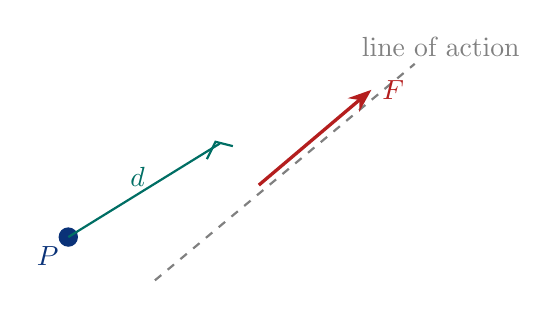
\begin{tikzpicture}[>=Stealth, scale=1.1]
  % Point P
  \filldraw[deepblue] (0,0) circle (3pt) node[below left] {$P$};
  
  % Line of action
  \draw[gray, dashed, thick] (1,-0.5) -- (4, 2);
  
  % Force arrow
  \draw[->, very thick, warmred] (2.2, 0.6) -- (3.5, 1.7) node[right] {$F$};
  
  % Perpendicular distance
  \draw[tealgreen, thick] (0,0) -- (1.75, 1.08);
  \draw[tealgreen, thick] (1.6, 0.9) -- (1.7, 1.1) -- (1.9, 1.05);
  \node[tealgreen] at (0.8, 0.7) {$d$};
  
  % Labels
  \node[gray] at (4.3, 2.2) {line of action};
  \node[warmred] at (4.1, 1.3) {};
\end{tikzpicture}
\end{center}

\subsection{The Perpendicular Distance}

The perpendicular distance $d$ is sometimes called the \textbf{moment arm} or \textbf{lever arm}. If the force $F$ makes angle $\theta$ with the line $PQ$ where $Q$ is any point on the line of action:
\[
  d = |PQ|\sin\theta
\]
Therefore $M = F \cdot |PQ|\sin\theta$, which is related to the cross product.

\begin{exmp}{Calculating a Moment}{}
A horizontal beam $AB$ of length $4\m$ rests on two supports. A force of $30\N$ acts vertically downward at a point $1.5\m$ from $A$. Find the moment of this force about (a) $A$, (b) $B$.

\medskip
(a) Moment about $A$: The perpendicular distance from $A$ to the line of action (vertical line through the point) is $1.5\m$. Moment $= 30 \times 1.5 = 45\Nm$ (clockwise, so $-45\Nm$ if anticlockwise is positive).

(b) Moment about $B$: The perpendicular distance from $B$ to the line of action is $4 - 1.5 = 2.5\m$. Moment $= 30 \times 2.5 = 75\Nm$ (anticlockwise about $B$, so $+75\Nm$).
\end{exmp}

\subsection{The Principle of Moments}

\begin{thm}{Principle of Moments (Varignon's Theorem)}{}
If a rigid body is in equilibrium:
\[
  \text{Sum of clockwise moments} = \text{Sum of anticlockwise moments}
\]
about any point. Equivalently, the \emph{algebraic sum} of all moments about any point is zero.

Moreover (Varignon's Theorem): the moment of a resultant force about any point equals the sum of the moments of its components about that point.
\end{thm}

\begin{intuitionbox}
The choice of pivot point is \emph{yours to make}. A clever choice of pivot eliminates unknown forces (reactions at pivots have zero moment about the pivot point), simplifying the algebra enormously.
\end{intuitionbox}

\section{Centres of Mass}

\subsection{What is the Centre of Mass?}

\begin{defn}{Centre of Mass}{}
The \textbf{centre of mass} of a system of particles is the point $G$ such that, if the entire mass were concentrated there, it would behave identically under forces. For a system of particles with masses $m_i$ at positions $\rvec_i$:
\[
  \bar{\rvec} = \frac{\sum m_i \rvec_i}{\sum m_i}
\]
In components:
\[
  \bar{x} = \frac{\sum m_i x_i}{\sum m_i}, \qquad \bar{y} = \frac{\sum m_i y_i}{\sum m_i}
\]
\end{defn}

\begin{intuitionbox}
The centre of mass is the \emph{weighted average position} of the mass. Heavy parts pull the centre of mass toward them. For a uniform body, the centre of mass coincides with the geometric centre (centroid).
\end{intuitionbox}

\subsection{Centres of Mass of Rods and Laminas}

\subsubsection{Uniform Bodies}
For uniform bodies, the centre of mass is at the geometric centre by symmetry:

\begin{center}
\begin{tabular}{llc}
\toprule
Shape & Centre of Mass & Distance from base \\
\midrule
Uniform rod & Midpoint & $\frac{L}{2}$ \\
Uniform rectangle & Centre & --- \\
Uniform circle/disc & Centre & --- \\
Uniform triangle & Centroid (intersection of medians) & $\frac{h}{3}$ from base \\
\bottomrule
\end{tabular}
\end{center}

\subsubsection{Composite Bodies}

For a body made of several parts, treat each part as a point mass at its own centre of mass.

\begin{exmp}{Composite Lamina}{}
A uniform rectangular lamina $ABCD$ has $AB = 4\m$ and $BC = 3\m$. A square of side $1\m$ is cut from corner $A$. Find the centre of mass of the remaining lamina.

\medskip
\textbf{Solution.} We use the \emph{negative mass method}: treat the original rectangle minus the cut square.

Let $A$ be the origin, with $AB$ along the $x$-axis.

\begin{center}
\begin{tabular}{lccc}
\toprule
Part & Mass (prop. to area) & $\bar{x}$ & $\bar{y}$ \\
\midrule
Full rectangle & $12$ & $2$ & $1.5$ \\
Cut square (subtract) & $-1$ & $0.5$ & $0.5$ \\
\midrule
Remainder & $11$ & ? & ? \\
\bottomrule
\end{tabular}
\end{center}

\[
  \bar{x} = \frac{12 \times 2 - 1 \times 0.5}{12 - 1} = \frac{24 - 0.5}{11} = \frac{23.5}{11} \approx 2.14\m
\]
\[
  \bar{y} = \frac{12 \times 1.5 - 1 \times 0.5}{11} = \frac{18 - 0.5}{11} = \frac{17.5}{11} \approx 1.59\m
\]
\end{exmp}

\subsection{Centre of Mass of Standard Shapes}

\begin{thm}{Centre of Mass of a Triangular Lamina}{}
For a uniform triangular lamina with vertices at $(x_1,y_1)$, $(x_2,y_2)$, $(x_3,y_3)$:
\[
  \bar{x} = \frac{x_1 + x_2 + x_3}{3}, \qquad \bar{y} = \frac{y_1 + y_2 + y_3}{3}
\]
The centre of mass lies at the \textbf{centroid} --- the intersection of the medians.
\end{thm}

\textbf{Derivation of the $\frac{1}{3}$ result:} Consider a triangle with base $b$ and height $h$, with the base on the $x$-axis. A horizontal strip at height $y$ has width proportional to $(1 - y/h)b$ and mass $dm = \rho b(1-y/h)\,dy$ where $\rho$ is surface mass density.

\[
  \bar{y} = \frac{\int_0^h y\,dm}{\int_0^h dm} = \frac{\int_0^h y(1-y/h)\,dy}{\int_0^h (1-y/h)\,dy}
\]
\[
  \text{Numerator} = \int_0^h y - \frac{y^2}{h}\,dy = \left[\frac{y^2}{2} - \frac{y^3}{3h}\right]_0^h = \frac{h^2}{2} - \frac{h^2}{3} = \frac{h^2}{6}
\]
\[
  \text{Denominator} = \int_0^h 1 - \frac{y}{h}\,dy = \left[y - \frac{y^2}{2h}\right]_0^h = h - \frac{h}{2} = \frac{h}{2}
\]
\[
  \therefore \bar{y} = \frac{h^2/6}{h/2} = \frac{h}{3}
\]
The centre of mass is $\frac{h}{3}$ above the base, confirming the centroid result.

\section{Centres of Mass of Solids}

\subsection{Solids of Revolution}

For three-dimensional solids, we use integration. The most important case is a \textbf{solid of revolution}: a solid formed by rotating a region about an axis.

\begin{thm}{Centre of Mass of a Solid of Revolution}{}
For a uniform solid formed by rotating $y = f(x)$ about the $x$-axis, from $x = a$ to $x = b$:
\[
  \bar{x} = \frac{\int_a^b x \cdot \pi[f(x)]^2\,dx}{\int_a^b \pi[f(x)]^2\,dx} = \frac{\int_a^b x[f(x)]^2\,dx}{\int_a^b [f(x)]^2\,dx}
\]
By symmetry, $\bar{y} = 0$.
\end{thm}

\begin{exmp}{Centre of Mass of a Solid Cone}{}
Find the centre of mass of a uniform solid cone of height $h$ and base radius $r$.

\medskip
\textbf{Setup.} Place the apex at the origin, axis along the $x$-axis. The cone is formed by rotating $y = \frac{r}{h}x$ (for $0 \leq x \leq h$) about the $x$-axis.

\[
  \bar{x} = \frac{\int_0^h x \left(\frac{r}{h}x\right)^2 dx}{\int_0^h \left(\frac{r}{h}x\right)^2 dx} = \frac{\frac{r^2}{h^2}\int_0^h x^3\,dx}{\frac{r^2}{h^2}\int_0^h x^2\,dx} = \frac{\int_0^h x^3\,dx}{\int_0^h x^2\,dx} = \frac{h^4/4}{h^3/3} = \frac{3h}{4}
\]

The centre of mass is $\frac{3h}{4}$ from the apex, or equivalently $\frac{h}{4}$ from the base.
\end{exmp}

\begin{exmp}{Centre of Mass of a Solid Hemisphere}{}
Find the centre of mass of a uniform solid hemisphere of radius $r$.

\medskip
\textbf{Setup.} Place the flat face at $x = 0$, curved surface facing $x > 0$. The hemisphere is $x^2 + y^2 \leq r^2$, $x \geq 0$, rotated about the $x$-axis using $y^2 = r^2 - x^2$.

\[
  \bar{x} = \frac{\int_0^r x(r^2-x^2)\,dx}{\int_0^r (r^2-x^2)\,dx}
\]
\[
  \text{Numerator} = \int_0^r (r^2x - x^3)\,dx = \left[\frac{r^2x^2}{2} - \frac{x^4}{4}\right]_0^r = \frac{r^4}{2} - \frac{r^4}{4} = \frac{r^4}{4}
\]
\[
  \text{Denominator} = \int_0^r (r^2 - x^2)\,dx = \left[r^2x - \frac{x^3}{3}\right]_0^r = r^3 - \frac{r^3}{3} = \frac{2r^3}{3}
\]
\[
  \bar{x} = \frac{r^4/4}{2r^3/3} = \frac{3r}{8}
\]

The centre of mass is $\frac{3r}{8}$ from the flat face.
\end{exmp}

\begin{center}
\begin{tabular}{ll}
\toprule
Solid & Distance of CoM from base \\
\midrule
Solid cone (height $h$) & $\frac{h}{4}$ from base \\
Solid hemisphere (radius $r$) & $\frac{3r}{8}$ from flat face \\
Hollow cone (height $h$) & $\frac{h}{3}$ from base \\
Hollow hemisphere (radius $r$) & $\frac{r}{2}$ from flat face \\
\bottomrule
\end{tabular}
\end{center}

\section{Objects in Equilibrium}

\subsection{Conditions for Equilibrium}

\begin{thm}{Conditions for Equilibrium of a Rigid Body}{}
A rigid body is in equilibrium if and only if:
\begin{enumerate}[label=(\roman*)]
  \item The vector sum of all forces is zero: $\sum \Fvec_i = \mathbf{0}$
  \item The sum of moments of all forces about any point is zero: $\sum M_i = 0$
\end{enumerate}
\end{thm}

For a two-dimensional problem this gives three scalar equations (two from force balance, one from moment balance) which can determine up to three unknowns.

\begin{exmp}{Beam with Support Reactions}{}
A uniform beam $AB$ of mass $20\kg$ and length $6\m$ rests on supports at $A$ and at a point $C$, $4\m$ from $A$. A load of $40\kg$ hangs from $B$. Find the reactions at $A$ and $C$.

\medskip
\textbf{Solution.} Let reactions be $R_A$ (at $A$) and $R_C$ (at $C$), both upward.

\textbf{Forces:} Weight of beam $= 20g$ at midpoint $3\m$ from $A$; Load $= 40g$ at $B$ ($6\m$ from $A$); $R_A$ at $A$; $R_C$ at $C$ ($4\m$ from $A$).

\textbf{Moments about $A$} (eliminates $R_A$):
\[
  R_C \times 4 = 20g \times 3 + 40g \times 6
\]
\[
  4R_C = 60g + 240g = 300g \implies R_C = 75g = 735\N
\]

\textbf{Vertical equilibrium:}
\[
  R_A + R_C = 20g + 40g = 60g
\]
\[
  R_A = 60g - 75g = -15g = -147\N
\]

The negative sign indicates $R_A$ acts \emph{downward} --- the support at $A$ must pull the beam down, i.e., the beam is pressing upward on the support. This means support $A$ is a clamp or fastening.
\end{exmp}

\subsection{Tilting and Toppling}

\begin{intuitionbox}
A body resting on a surface will \textbf{tilt} (rotate about an edge) when the vertical line through its centre of mass passes outside its base. This is the fundamental principle behind why objects fall over --- the moment due to gravity is no longer balanced by the reaction.
\end{intuitionbox}

\begin{exmp}{When Does a Box Tilt?}{}
A uniform rectangular box of width $2\m$ and height $4\m$ rests on a horizontal surface. The box is tilted by a horizontal force applied at the top. At what tilt angle does it topple?

\textbf{Solution.} The box will topple when the centre of mass is directly above the pivoting bottom corner.

The centre of mass is at the geometric centre: $1\m$ from the side, $2\m$ above the base. When the box tilts at angle $\theta$ from the vertical, the condition for toppling is when the CoM is vertically above the pivot corner.

By geometry, the critical angle satisfies:
\[
  \tan\theta = \frac{1}{2} \implies \theta = \arctan(0.5) \approx 26.6^\circ
\]
\end{exmp}

\subsection{Friction and Equilibrium}

When a body rests on a rough surface, friction may act. We must check both \emph{sliding} (net force) and \emph{toppling} (net moment).

\begin{exmp}{Ladder Against a Wall}{}
A uniform ladder of mass $m$ and length $2a$ rests with its base on rough horizontal ground (coefficient of friction $\mu$) and its top against a smooth vertical wall. The ladder makes angle $\alpha$ with the ground. Find the minimum $\mu$ for equilibrium.

\medskip
\textbf{Solution.} Forces acting: weight $mg$ downward at midpoint; normal reaction $N_W$ horizontal from wall; normal reaction $N_G$ vertical from ground; friction $F$ horizontal at base (away from wall).

\textbf{Horizontal equilibrium:} $F = N_W$

\textbf{Vertical equilibrium:} $N_G = mg$

\textbf{Moments about the base} (eliminates $F$ and $N_G$):
\[
  N_W \times 2a\sin\alpha = mg \times a\cos\alpha
\]
\[
  N_W = \frac{mg\cos\alpha}{2\sin\alpha} = \frac{mg}{2}\cot\alpha
\]

For no sliding: $F \leq \mu N_G$, i.e., $N_W \leq \mu mg$:
\[
  \frac{mg}{2}\cot\alpha \leq \mu mg \implies \mu \geq \frac{\cot\alpha}{2} = \frac{\cos\alpha}{2\sin\alpha}
\]

As $\alpha$ decreases (ladder more horizontal), $\cot\alpha$ increases, requiring greater $\mu$. This matches intuition: a nearly flat ladder slides more easily.
\end{exmp}

\section{Connections and Advanced Ideas}

\begin{explorationbox}
\textbf{Torque and Angular Momentum (University Level).}
At university, the moment of a force is generalised to the \textbf{torque} $\boldsymbol{\tau} = \rvec \times \Fvec$ (cross product). Newton's second law for rotation becomes:
\[
  \boldsymbol{\tau} = I\boldsymbol{\alpha}
\]
where $I$ is the \textbf{moment of inertia} and $\boldsymbol{\alpha}$ is angular acceleration. The moment of inertia $I = \sum m_i r_i^2$ (for discrete masses) or $I = \int r^2\,dm$ (for continuous bodies) plays the role of mass in rotational dynamics.
\end{explorationbox}

\begin{summarybox}[Chapter 14 Summary: Equilibrium of a Rigid Body]
\begin{itemize}[leftmargin=1.5em]
  \item Moment $= F \times d$ (perpendicular distance); units N\,m
  \item Principle of Moments: for equilibrium, algebraic sum of moments about any point $= 0$
  \item Centre of mass: $\bar{x} = \frac{\sum m_i x_i}{\sum m_i}$ (weighted mean position)
  \item Standard CoM positions: triangle ($h/3$ from base), cone ($h/4$ from base), hemisphere ($3r/8$ from flat face)
  \item Equilibrium requires: (i) $\sum F = 0$; (ii) $\sum M = 0$ about any point
  \item Choose pivot wisely to eliminate unknown reactions
  \item A body topples when vertical line through CoM passes outside the support base
\end{itemize}
\end{summarybox}

% =====================================================================
% =====================================================================
%  CHAPTER 15: CIRCULAR MOTION
% =====================================================================
% =====================================================================
\chapter{Circular Motion}

\section{Introduction}

\subsection{The Physics of Circular Motion}

Circular motion is motion along a circular path. What makes it fascinating is this: a particle moving in a circle at \emph{constant speed} is still \emph{accelerating}. How can something move at constant speed and yet accelerate?

The answer is that acceleration is the rate of change of \emph{velocity}, not speed. Velocity is a vector. Even if the magnitude (speed) stays constant, the direction changes continuously --- and any change in direction is an acceleration.

\begin{intuitionbox}
Swing a ball on a string in a circle. You feel the string pulling outward (from your perspective). But by Newton's third law, the string pulls the ball \emph{inward}. This inward pull is the \textbf{centripetal force} --- it constantly changes the direction of the ball's velocity without changing its speed.

``Centripetal'' comes from Latin: \emph{centrum} (centre) + \emph{petere} (to seek). The force always points toward the centre.
\end{intuitionbox}

\section{Kinematics of Circular Motion}

\subsection{Angular Velocity}

\begin{defn}{Angular Velocity}{}
For a particle moving in a circle of radius $r$, the \textbf{angular velocity} $\omega$ is the rate of change of the angle $\theta$ subtended at the centre:
\[
  \omega = \dv{\theta}{t}
\]
Units: radians per second ($\mathrm{rad\,s}^{-1}$). For uniform circular motion, $\omega$ is constant.

The relationship between linear speed $v$ and angular velocity:
\[
  v = r\omega
\]
\end{defn}

\begin{defn}{Period and Frequency}{}
The \textbf{period} $T$ is the time for one complete revolution: $T = \dfrac{2\pi}{\omega}$.

The \textbf{frequency} $f$ is the number of revolutions per second: $f = \dfrac{1}{T} = \dfrac{\omega}{2\pi}$.
\end{defn}

\subsection{Centripetal Acceleration}

\begin{thm}{Centripetal Acceleration}{}
A particle moving with speed $v$ in a circle of radius $r$ has acceleration directed toward the centre of magnitude:
\[
  a = \frac{v^2}{r} = r\omega^2 = v\omega
\]
\end{thm}

\textbf{Derivation.} Let the particle be at angle $\theta = \omega t$ from the positive $x$-axis. Its position is:
\[
  \rvec = r\cos(\omega t)\,\ii + r\sin(\omega t)\,\jj
\]
Velocity:
\[
  \vvec = \dv{\rvec}{t} = -r\omega\sin(\omega t)\,\ii + r\omega\cos(\omega t)\,\jj
\]
Acceleration:
\[
  \avec = \dv{\vvec}{t} = -r\omega^2\cos(\omega t)\,\ii - r\omega^2\sin(\omega t)\,\jj = -\omega^2\rvec
\]

The acceleration is $-\omega^2\rvec$: it points \emph{toward the centre} (opposite to $\rvec$) with magnitude $\omega^2 r = v^2/r$. This is the centripetal acceleration.

\begin{center}
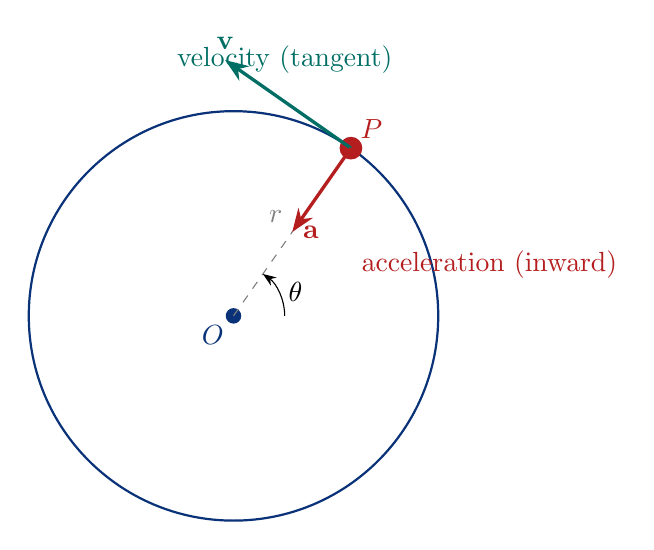
\begin{tikzpicture}[>=Stealth, scale=1.3]
  % Circle
  \draw[thick, deepblue] (0,0) circle (2);
  \filldraw[deepblue] (0,0) circle (2pt) node[below left] {$O$};
  
  % Particle position
  \def\angle{55}
  \coordinate (P) at ({2*cos(\angle)}, {2*sin(\angle)});
  \filldraw[warmred] (P) circle (3pt) node[above right] {$P$};
  
  % Radius
  \draw[gray, dashed] (0,0) -- (P) node[midway, above left] {$r$};
  
  % Velocity (tangential)
  \draw[->, very thick, tealgreen] (P) -- ++({-1.5*sin(\angle)}, {1.5*cos(\angle)}) node[above] {$\vvec$};
  
  % Acceleration (centripetal, toward centre)
  \draw[->, very thick, warmred] (P) -- ++({-1.0*cos(\angle)}, {-1.0*sin(\angle)}) node[right] {$\avec$};
  
  % Angle
  \draw[->] (0.5,0) arc (0:\angle:0.5) node[midway, right] {$\theta$};
  
  % Labels
  \node[tealgreen] at (0.5, 2.5) {velocity (tangent)};
  \node[warmred] at (2.5, 0.5) {acceleration (inward)};
\end{tikzpicture}
\end{center}

\subsection{Centripetal Force}

\begin{defn}{Centripetal Force}{}
By Newton's second law, the net force required to maintain circular motion is:
\[
  F = ma = \frac{mv^2}{r} = mr\omega^2
\]
This force must be directed toward the centre. It is provided by whatever physical mechanism is relevant: tension in a string, friction on a car tyre, gravity on an orbiting planet, normal force on a banked road.
\end{defn}

\begin{warningbox}
\textbf{``Centrifugal force'' is not a real force!} In an inertial frame, there is no outward ``centrifugal force''. What we experience as the sensation of being pushed outward is simply inertia --- our body's tendency to continue in a straight line. The centrifugal force is a \emph{fictitious force} that appears only in the rotating reference frame. Never include it in force diagrams in an inertial frame.
\end{warningbox}

\section{Horizontal Circles}

\subsection{Particle on a String --- Conical Pendulum}

A classic example: a particle $P$ of mass $m$ is attached to a string of length $l$ and moves in a horizontal circle. The string makes angle $\theta$ with the vertical. This is the \textbf{conical pendulum}.

\begin{center}
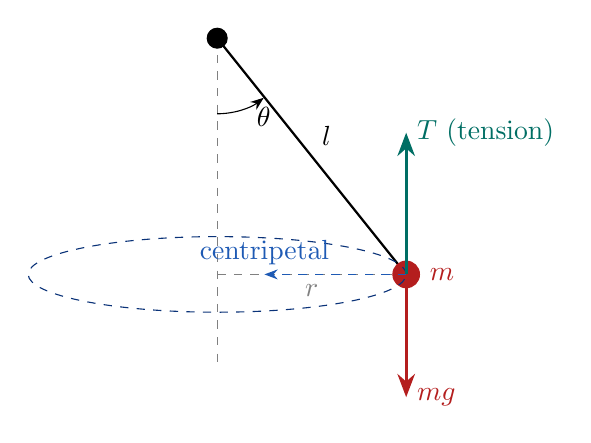
\begin{tikzpicture}[>=Stealth, scale=1.2]
  % Vertical string / axis
  \draw[gray, dashed] (0,0) -- (0,-3.5);
  \filldraw[black] (0,0) circle (3pt);
  
  % String
  \draw[thick] (0,0) -- (2,-2.5) node[midway, above right] {$l$};
  
  % Particle
  \filldraw[warmred] (2,-2.5) circle (4pt) node[right=5pt] {$m$};
  
  % Circle (horizontal)
  \draw[dashed, deepblue] (0,-2.5) ellipse (2 and 0.4);
  \draw[dashed, gray] (0,-2.5) -- (2,-2.5) node[midway, below] {$r$};
  
  % Forces
  \draw[->, very thick, tealgreen] (2,-2.5) -- (2,-1.0) node[right] {$T$ (tension)};
  \draw[->, very thick, warmred] (2,-2.5) -- (2,-3.8) node[right] {$mg$};
  
  % Horizontal arrow (centripetal direction)
  \draw[->, dashed, midblue] (2,-2.5) -- (0.5,-2.5) node[above] {centripetal};
  
  % Angle
  \draw[->] (0,-0.8) arc (270:308:0.8) node[below] {$\theta$};
\end{tikzpicture}
\end{center}

\textbf{Analysis.} Resolving forces:

Vertical: $T\cos\theta = mg \implies T = \dfrac{mg}{\cos\theta}$

Horizontal (centripetal): $T\sin\theta = \dfrac{mv^2}{r}$

Dividing: $\tan\theta = \dfrac{v^2}{rg}$

Since $r = l\sin\theta$:
\[
  \tan\theta = \frac{v^2}{lg\sin\theta} \implies v^2 = lg\sin\theta\tan\theta
\]

Period:
\[
  T = \frac{2\pi r}{v} = 2\pi\sqrt{\frac{l\cos\theta}{g}}
\]

\begin{intuitionbox}
Notice that the period $T = 2\pi\sqrt{\frac{l\cos\theta}{g}}$ looks like the formula for a simple pendulum: $T = 2\pi\sqrt{L/g}$ where $L = l\cos\theta$ is the \emph{vertical} length of the string. This is not a coincidence --- both involve the balance of gravity and the requirement for circular/oscillatory motion.
\end{intuitionbox}

\begin{exmp}{Conical Pendulum Problem}{}
A particle moves in a horizontal circle at the end of a string of length $0.8\m$. The string makes angle $30^\circ$ with the vertical. Find (a) the speed of the particle, (b) the period, (c) the tension.

\medskip
(a) $r = l\sin 30^\circ = 0.8 \times 0.5 = 0.4\m$

$v^2 = rg\tan\theta = 0.4 \times 9.8 \times \tan 30^\circ = 0.4 \times 9.8 \times \frac{1}{\sqrt{3}} \approx 2.263$

$v \approx 1.50\ms$

(b) $T = 2\pi\sqrt{\frac{l\cos\theta}{g}} = 2\pi\sqrt{\frac{0.8\cos 30^\circ}{9.8}} = 2\pi\sqrt{0.0707} \approx 1.67\,\mathrm{s}$

(c) $T_{\text{tension}} = \frac{mg}{\cos\theta} = \frac{m \times 9.8}{\cos 30^\circ} = \frac{9.8m}{\sqrt{3}/2} = \frac{19.6m}{\sqrt{3}} \approx 11.32m\,\N$
\end{exmp}

\subsection{Banked Tracks}

On a banked road (inclined at angle $\theta$ to horizontal), a vehicle can navigate a corner without friction.

\textbf{Analysis.} The only forces are weight $mg$ and normal reaction $N$ (perpendicular to road, no friction).

Vertical: $N\cos\theta = mg$

Horizontal (centripetal): $N\sin\theta = \dfrac{mv^2}{r}$

Dividing:
\[
  \tan\theta = \frac{v^2}{rg} \implies v = \sqrt{rg\tan\theta}
\]

This is the \textbf{design speed} of the banked road. For this speed, no friction is needed.

\section{The 3-Dimensional Case}

\subsection{Motion in Space}

The same centripetal acceleration formula applies in three dimensions. For a particle constrained to move on the surface of a cone, in a helical path, or on a sphere, the key is to identify the relevant circle at each moment.

\begin{exmp}{Particle on Inside of a Cone}{}
A smooth hollow cone has half-angle $\alpha$ and its axis vertical (apex down). A particle of mass $m$ moves in a horizontal circle on the inner surface. If the circle has radius $r$, find the speed.

The normal reaction $N$ acts perpendicular to the cone surface (at angle $\alpha$ from horizontal).

Vertical: $N\sin\alpha = mg \implies N = \frac{mg}{\sin\alpha}$

Horizontal: $N\cos\alpha = \frac{mv^2}{r}$

\[
  v^2 = \frac{Nr\cos\alpha}{m} = \frac{mg\cos\alpha \cdot r}{\sin\alpha \cdot m} = rg\cot\alpha
\]

\[
  v = \sqrt{rg\cot\alpha}
\]
\end{exmp}

\section{Vertical Circles}

\subsection{Why Vertical Circles Are Different}

In vertical circles, the speed changes (gravity does work as the particle moves up or down), so we must use energy conservation to find the speed at each point, then Newton's second law to find the tension or normal reaction.

\begin{intuitionbox}
The critical question in vertical circle problems is: \emph{does the particle maintain contact with the surface / remain taut on the string throughout?} The answer depends on whether the speed is sufficient at the top of the circle to provide the centripetal force needed, even with gravity helping.
\end{intuitionbox}

\subsection{Particle on the Inside of a Circle (String)}

Consider a particle on a string of length $r$, moving in a vertical circle. The string goes slack when the tension $T = 0$.

At any point making angle $\theta$ with the bottom, using energy conservation from the bottom:
\[
  \tfrac{1}{2}mv^2 = \tfrac{1}{2}mv_{\text{bottom}}^2 - mgr(1 - \cos\theta)
\]
\[
  v^2 = v_0^2 - 2gr(1-\cos\theta)
\]

Applying Newton's second law along the string (centripetal direction, toward centre):
\[
  T - mg\cos\phi = \frac{mv^2}{r}
\]
where $\phi$ is the angle from the upward vertical (so at the top $\phi = 0$, $\cos\phi = 1$).

\textbf{At the top ($\phi = 0$, i.e., highest point):}
\[
  T + mg = \frac{mv_{\text{top}}^2}{r} \quad \text{(both $T$ and $mg$ point toward centre)}
\]

Wait, more carefully: At the top, the centre is directly below, so centripetal direction is downward. Both $T$ (along string toward centre) and $mg$ (downward = toward centre) contribute:
\[
  T + mg = \frac{mv_{\text{top}}^2}{r}
\]

For the string to remain taut: $T \geq 0 \implies v_{\text{top}}^2 \geq gr$, i.e., $v_{\text{top}} \geq \sqrt{gr}$.

Using energy conservation from bottom to top (height change $= 2r$):
\[
  v_{\text{top}}^2 = v_0^2 - 4gr
\]

Condition for complete circle: $v_0^2 - 4gr \geq gr \implies v_0 \geq \sqrt{5gr}$.

\begin{thm}{Condition for Complete Vertical Circle (String)}{}
A particle on a string of length $r$ will complete a full vertical circle if and only if:
\[
  v_0 \geq \sqrt{5gr}
\]
where $v_0$ is the speed at the bottom. The minimum speed at the top is $\sqrt{gr}$.
\end{thm}

\subsection{Particle on the Outside of a Circle (Surface)}

For a particle on the \emph{outside} of a smooth sphere of radius $r$, the normal reaction can only push outward (never pull inward). The particle leaves the surface when $N = 0$.

At angle $\theta$ from the top:

Energy conservation (from top, starting with speed $v_{\text{top}}$, height fallen $= r - r\cos\theta$):
\[
  v^2 = v_{\text{top}}^2 + 2gr(1-\cos\theta)
\]

Newton's second law (centripetal, toward centre = downward component at angle $\theta$ from top):
\[
  mg\cos\theta - N = \frac{mv^2}{r}
\]

Setting $N = 0$:
\[
  mg\cos\theta = \frac{mv^2}{r} \implies v^2 = gr\cos\theta
\]

Combining with energy equation:
\[
  gr\cos\theta = v_{\text{top}}^2 + 2gr(1 - \cos\theta)
\]
If the particle starts from rest at the top ($v_{\text{top}} = 0$):
\[
  gr\cos\theta = 2gr(1-\cos\theta) \implies \cos\theta = 2 - 2\cos\theta \implies 3\cos\theta = 2 \implies \cos\theta = \frac{2}{3}
\]
\[
  \theta = \arccos\!\left(\tfrac{2}{3}\right) \approx 48.2^\circ
\]

The particle leaves the sphere at this angle from the top.

\begin{exmp}{Challenging Vertical Circle}{}
A particle of mass $m$ is attached to a string of length $r$ and moves in a vertical circle. At the bottom, it has speed $4\sqrt{gr}$. Find (a) the speed at the top, (b) the tension at the top, (c) whether it completes the circle.

\medskip
(a) $v_{\text{top}}^2 = (4\sqrt{gr})^2 - 4gr = 16gr - 4gr = 12gr$, so $v_{\text{top}} = 2\sqrt{3gr}$.

(b) At the top: $T + mg = \frac{mv_{\text{top}}^2}{r} = \frac{m \times 12gr}{r} = 12mg$

$T = 12mg - mg = 11mg$

(c) Since $v_0 = 4\sqrt{gr} > \sqrt{5gr}$ (as $16 > 5$), the particle \emph{does} complete the circle.
\end{exmp}

\section{Common Mistakes in Circular Motion}

\begin{warningbox}
\textbf{Centripetal direction changes.} The centripetal direction is always \emph{toward the centre} of the circle, and this direction changes as the particle moves. At the top of a vertical circle, centripetal is downward. At the side, centripetal is horizontal. Always identify the current position before writing Newton's second law.
\end{warningbox}

\begin{examtrap}
\textbf{Energy conservation in vertical circles.}
Students sometimes apply $v^2 = u^2 + 2as$ (constant acceleration) to vertical circles. This is wrong: the centripetal acceleration is not constant in direction. The correct approach is the work-energy theorem / energy conservation (which gives the speed), then Newton's second law (which gives forces).
\end{examtrap}

\begin{warningbox}
\textbf{String vs. surface.}
For a string: tension can only pull (never push), so the string goes slack when $T = 0$.
For a surface: normal reaction can only push (never pull), so the particle leaves the surface when $N = 0$.
These give different critical conditions.
\end{warningbox}

\section{Advanced: Non-Uniform Circular Motion}

If a particle moves in a circle with varying speed, there are \emph{two} components of acceleration:
\begin{itemize}[leftmargin=2em]
  \item \textbf{Centripetal}: $a_c = v^2/r$ directed toward centre
  \item \textbf{Tangential}: $a_t = \dot{v}$ along the tangent
\end{itemize}
The total acceleration is $a = \sqrt{a_c^2 + a_t^2}$.

\begin{summarybox}[Chapter 15 Summary: Circular Motion]
\begin{itemize}[leftmargin=1.5em]
  \item Angular velocity: $\omega = d\theta/dt$; $v = r\omega$; $T = 2\pi/\omega$
  \item Centripetal acceleration: $a = v^2/r = r\omega^2$ (toward centre)
  \item Centripetal force: $F = mv^2/r = mr\omega^2$ (provided by real forces)
  \item Conical pendulum: $T = 2\pi\sqrt{l\cos\theta/g}$; $v = \sqrt{rg\tan\theta}$
  \item Banked roads: design speed $v = \sqrt{rg\tan\theta}$
  \item Vertical circles (string): minimum bottom speed $\sqrt{5gr}$; min top speed $\sqrt{gr}$
  \item Particle leaves sphere: at $\cos\theta = 2/3$ from top (starting from rest)
  \item Always use energy conservation for speed, Newton's second law for forces
\end{itemize}
\end{summarybox}

% =====================================================================
% =====================================================================
%  CHAPTER 16: HOOKE'S LAW
% =====================================================================
% =====================================================================
\chapter{Hooke's Law}

\section{Introduction}

\subsection{Springs and Elasticity}

When you stretch a rubber band and release it, it snaps back. When you compress a spring, it pushes back. This restorative behaviour is called \textbf{elasticity}. In mechanics, elastic strings and springs are essential models for understanding oscillations, collisions, energy storage, and vibrations.

\begin{intuitionbox}
The deeper reason that springs obey a simple linear law is that, at the atomic level, the bonds between atoms are like tiny springs. When stretched slightly, the restoring force is proportional to the displacement --- this is a general feature of any system near a stable equilibrium (Taylor expansion of the potential energy).
\end{intuitionbox}

\begin{historicalbox}
\textbf{Robert Hooke} (1635--1703), a contemporary and rival of Newton, discovered the law of springs in 1660. He first published it as an anagram: \emph{ceiiinosssttuv} (the letters of \emph{ut tensio sic vis}, Latin for ``as the extension, so the force''). He revealed the anagram only in 1678. Hooke was also the first to use the word ``cell'' in biology, after viewing cork through his microscope.
\end{historicalbox}

\section{Hooke's Law}

\subsection{The Law}

\begin{thm}{Hooke's Law}{}
For an elastic string or spring with \textbf{natural length} $l_0$ and \textbf{modulus of elasticity} $\lambda$ (or spring constant $k$):

The tension (for a string) or restoring force (for a spring) when extended by $x$ is:
\[
  \boxed{T = \frac{\lambda x}{l_0} = kx}
\]
where $k = \lambda/l_0$ is the spring constant (force per unit extension), units $\mathrm{N\,m}^{-1}$.

For a spring: compression by $x$ produces thrust $T = kx$ (outward).
\end{thm}

\begin{defn}{Natural Length and Extension}{}
The \textbf{natural length} $l_0$ is the length of the string/spring when no force is applied.
The \textbf{extension} $x = l - l_0$ where $l$ is the current length. For a compressed spring, $x < 0$ (compression).
The \textbf{modulus of elasticity} $\lambda$ has units of Newtons; it represents the force required to double the natural length.
\end{defn}

\subsection{Physical Interpretation}

The modulus $\lambda = kl_0$. A stiffer spring (large $\lambda$) requires more force for the same extension. A longer spring (large $l_0$) requires less force per unit extension.

\begin{center}
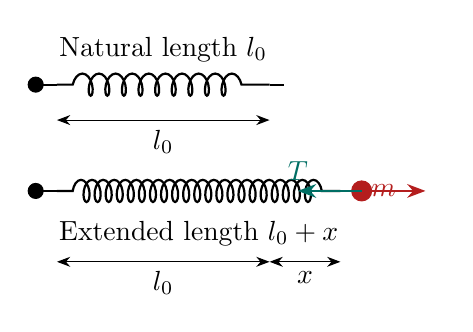
\begin{tikzpicture}[>=Stealth, scale=0.9]
  % Natural length spring
  \draw[thick, decoration={coil, segment length=6pt, amplitude=4pt, pre length=0.2cm, post length=0.2cm}, decorate] 
    (0,1) -- (3,1);
  \draw[thick] (-0.2,1) -- (0,1);
  \draw[thick] (3,1) -- (3.2,1);
  \filldraw[black] (-0.3,1) circle (3pt);
  \node at (1.5, 1.5) {Natural length $l_0$};
  \draw[<->] (0, 0.5) -- (3, 0.5) node[midway, below] {$l_0$};

  % Extended spring
  \draw[thick, decoration={coil, segment length=4pt, amplitude=4pt, pre length=0.2cm, post length=0.2cm}, decorate] 
    (0,-0.5) -- (4,-0.5);
  \draw[thick] (-0.2,-0.5) -- (0,-0.5);
  \draw[thick] (4,-0.5) -- (4.2,-0.5);
  \filldraw[black] (-0.3,-0.5) circle (3pt);
  \filldraw[warmred] (4.3,-0.5) circle (4pt) node[right] {$m$};
  \draw[->, thick, warmred] (4.3,-0.5) -- (5.2,-0.5) node[right] {};
  \draw[->, thick, tealgreen] (4.3,-0.5) -- (3.4,-0.5) node[above] {$T$};
  \node at (2, -1.1) {Extended length $l_0 + x$};
  \draw[<->] (0,-1.5) -- (3,-1.5) node[midway, below] {$l_0$};
  \draw[<->] (3,-1.5) -- (4,-1.5) node[midway, below] {$x$};
\end{tikzpicture}
\end{center}

\section{Elastic Potential Energy}

\subsection{Deriving the Energy Formula}

When a spring is extended or compressed, energy is stored in it as \textbf{elastic potential energy (EPE)}. We derive this by calculating the work done against the restoring force.

To extend the spring from extension $0$ to $x$, the applied force equals the spring force: $F = kx' = \frac{\lambda x'}{l_0}$.

\[
  W = \int_0^x F\,dx' = \int_0^x \frac{\lambda x'}{l_0}\,dx' = \frac{\lambda}{l_0} \cdot \frac{x^2}{2}
\]

\begin{thm}{Elastic Potential Energy}{}
The elastic potential energy stored in a string/spring with modulus $\lambda$, natural length $l_0$, and extension $x$ is:
\[
  \boxed{E_{\text{EPE}} = \frac{\lambda x^2}{2l_0} = \frac{kx^2}{2}}
\]
\end{thm}

\begin{intuitionbox}
This is the area of the triangle under the force-extension graph ($F = kx$, linear). Alternatively, it is $\frac{1}{2}Tx$ where $T = kx$ is the tension. This formula is the elastic analogue of gravitational PE ($mgh$) --- it represents energy waiting to be released.
\end{intuitionbox}

\section{The Work--Energy Principle with Elastic Forces}

\begin{thm}{Conservation of Energy with Elastic Potential Energy}{}
For a system involving gravity, kinetic energy, and elastic forces:
\[
  \Delta KE + \Delta GPE + \Delta EPE = W_{\text{non-conservative}}
\]
If there are no friction or non-conservative forces:
\[
  KE + GPE + EPE = \text{constant}
\]
i.e., $\tfrac{1}{2}mv^2 + mgh + \tfrac{\lambda x^2}{2l_0} = \text{constant}$
\end{thm}

\begin{exmp}{Particle on Spring on Smooth Table}{}
A particle of mass $0.3\kg$ is attached to a spring (natural length $0.5\m$, $k = 40\,\mathrm{Nm}^{-1}$) on a smooth horizontal table. The particle is pulled so the spring has extension $0.2\m$ and released from rest. Find the speed when the extension is $0.1\m$.

\medskip
\textbf{Solution.} No gravity changes (horizontal), no friction. Energy conservation:
\[
  \tfrac{1}{2}mv_1^2 + \tfrac{1}{2}kx_1^2 = \tfrac{1}{2}mv_2^2 + \tfrac{1}{2}kx_2^2
\]
\[
  0 + \tfrac{1}{2}(40)(0.2)^2 = \tfrac{1}{2}(0.3)v^2 + \tfrac{1}{2}(40)(0.1)^2
\]
\[
  0.8 = 0.15v^2 + 0.2
\]
\[
  0.15v^2 = 0.6 \implies v^2 = 4 \implies v = 2\ms
\]
\end{exmp}

\begin{exmp}{Vertical Spring}{}
A particle of mass $2\kg$ hangs on a spring with natural length $1\m$ and $\lambda = 40\N$. Find the equilibrium extension. The particle is then pulled down a further $0.3\m$ and released. Find the speed when passing through equilibrium.

\medskip
\textbf{Part 1: Equilibrium extension.}
At equilibrium: $T = mg \implies \frac{\lambda x_0}{l_0} = mg \implies \frac{40x_0}{1} = 2 \times 9.8 \implies x_0 = 0.49\m$.

\textbf{Part 2: Speed at equilibrium.}

Take the equilibrium position as reference. The particle starts $0.3\m$ below, at extension $x_0 + 0.3 = 0.79\m$, from rest.

Energy conservation (taking equilibrium as $h = 0$):
\[
  KE_i + GPE_i + EPE_i = KE_f + GPE_f + EPE_f
\]
\[
  0 + mg(-0.3) + \tfrac{\lambda(0.79)^2}{2l_0} = \tfrac{1}{2}mv^2 + 0 + \tfrac{\lambda(0.49)^2}{2l_0}
\]

Using $\lambda = 40$, $l_0 = 1$, $m = 2$:
\[
  -2(9.8)(0.3) + \tfrac{40(0.79)^2}{2} = \tfrac{1}{2}(2)v^2 + \tfrac{40(0.49)^2}{2}
\]
\[
  -5.88 + 12.482 = v^2 + 4.802
\]
\[
  v^2 = 12.482 - 5.88 - 4.802 = 1.8 \implies v = \sqrt{1.8} \approx 1.34\ms
\]
\end{exmp}

\begin{exmp}{Most Challenging --- Particle Falls onto Spring}{}
A particle of mass $m$ falls from rest at height $H$ above the top of a vertical spring (natural length $l_0$, spring constant $k$). Find the maximum compression of the spring.

\medskip
\textbf{Solution.} Let the maximum compression be $d$. Energy conservation (taking initial position of particle as reference, downward positive):

The particle falls a total distance of $H + l_0 + d$ (falls $H$ before touching, then compresses spring by $d$ --- but the top of the spring is at natural length, so falls $H + d$). 

Actually: particle falls distance $H + d$ from when it touches the spring; compression $= d$.

Energy conservation from start to maximum compression:
\[
  mg(H + d) = \tfrac{1}{2}kd^2
\]
(all gravitational PE converts to elastic PE; KE = 0 at both start and maximum compression)

\[
  \tfrac{1}{2}kd^2 - mgd - mgH = 0
\]
\[
  d = \frac{mg \pm \sqrt{(mg)^2 + 2kmgH}}{k} = \frac{mg}{k}\left(1 + \sqrt{1 + \frac{2kH}{mg}}\right)
\]
(taking positive root for maximum compression).
\end{exmp}

\section{Simple Harmonic Motion Preview}

\begin{explorationbox}
A particle of mass $m$ on a spring of constant $k$, displaced by $x$ from equilibrium, satisfies:
\[
  m\ddot{x} = -kx \implies \ddot{x} = -\omega^2 x, \quad \omega = \sqrt{k/m}
\]
This is \textbf{Simple Harmonic Motion} (SHM), the most important oscillatory equation in physics. The solution is $x = A\cos(\omega t + \phi)$, a sinusoidal oscillation with angular frequency $\omega = \sqrt{k/m}$ and period $T = 2\pi\sqrt{m/k}$.

This connects Hooke's Law directly to the study of waves, resonance, and quantum mechanics (the quantum harmonic oscillator is the hydrogen atom of quantum physics).
\end{explorationbox}

\begin{summarybox}[Chapter 16 Summary: Hooke's Law]
\begin{itemize}[leftmargin=1.5em]
  \item Hooke's Law: $T = \frac{\lambda x}{l_0} = kx$ ($\lambda$ = modulus, $l_0$ = natural length, $x$ = extension)
  \item Elastic strings only pull (tension); springs can push or pull
  \item Elastic PE: $E = \frac{\lambda x^2}{2l_0} = \frac{1}{2}kx^2$
  \item Energy conservation: $KE + GPE + EPE = $ const (no friction)
  \item Equilibrium of hanging particle: $kx_0 = mg$
  \item Modulus $\lambda = kl_0$: the force to double the natural length
\end{itemize}
\end{summarybox}

% =====================================================================
% =====================================================================
%  CHAPTER 17: LINEAR MOTION UNDER A VARIABLE FORCE
% =====================================================================
% =====================================================================
\chapter{Linear Motion Under a Variable Force}

\section{Introduction}

In Chapters 1--12, forces were constant (or we used $F = ma$ with constant $a$, giving SUVAT). In the real world, forces vary. Air resistance depends on speed. The gravitational force between planets varies with distance. A rocket engine burns fuel and changes mass. Elastic forces grow with displacement.

This chapter teaches us to handle \textbf{variable forces} using calculus, providing the foundation for more advanced dynamics.

\begin{intuitionbox}
Newton's second law is really a differential equation: $F(x, v, t) = m\ddot{x}$. When $F$ is constant, the ODE is trivial --- SUVAT. When $F$ varies, we must integrate the ODE. The method depends on whether $F$ depends on $t$, $v$, or $x$ (or combinations).
\end{intuitionbox}

\section{Acceleration as a Function of Time}

\subsection{The Method}

If $F = F(t)$, then $a = F(t)/m = f(t)$.

To find velocity: $v = \int a\,dt + C$

To find displacement: $x = \int v\,dt + C$

\begin{exmp}{Force Varying with Time}{}
A particle of mass $2\kg$ starts from rest at the origin. A force $F = 6t - 4\,\N$ acts on it ($t \geq 0$). Find the velocity and position at time $t$.

\medskip
$a = F/m = (6t-4)/2 = 3t - 2$

$v = \int (3t-2)\,dt = \frac{3t^2}{2} - 2t + C$

At $t = 0$: $v = 0 \implies C = 0$. So $v = \frac{3t^2}{2} - 2t$.

$x = \int v\,dt = \frac{t^3}{2} - t^2 + D$

At $t = 0$: $x = 0 \implies D = 0$. So $x = \frac{t^3}{2} - t^2$.

\textbf{Note:} The particle is momentarily at rest when $v = 0$: $\frac{3t^2}{2} - 2t = t(\frac{3t}{2}-2) = 0 \implies t = 0$ or $t = \frac{4}{3}$.
\end{exmp}

\begin{exmp}{Challenging --- Rocket Motion}{}
A rocket has initial mass $m_0$ (including fuel) and burns fuel at rate $\mu\,\mathrm{kg\,s}^{-1}$. The exhaust speed relative to the rocket is $v_e$. Neglecting gravity, the thrust is $F = \mu v_e = $ constant. But the mass is $m(t) = m_0 - \mu t$.

Newton's second law: $F = m(t)\,a$:
\[
  \mu v_e = (m_0 - \mu t)\dv{v}{t}
\]
\[
  \dv{v}{t} = \frac{\mu v_e}{m_0 - \mu t}
\]
\[
  v = \int_0^t \frac{\mu v_e}{m_0 - \mu s}\,ds = v_e\left[-\ln(m_0 - \mu s)\right]_0^t = v_e\ln\frac{m_0}{m_0 - \mu t}
\]

This is the \textbf{Tsiolkovsky rocket equation}. It shows that speed increases logarithmically with the ratio of initial to current mass.
\end{exmp}

\section{Acceleration as a Function of Displacement}

\subsection{The Technique: $a = v\dv{v}{x}$}

When $F = F(x)$ (force depends on position), we use the chain rule:
\[
  a = \dv{v}{t} = \dv{v}{x}\cdot\dv{x}{t} = v\dv{v}{x}
\]

So $F(x) = mv\dv{v}{x}$.

Separating variables: $v\,dv = \frac{F(x)}{m}\,dx$

Integrating both sides: $\tfrac{1}{2}v^2 = \int \frac{F(x)}{m}\,dx + C$

\begin{intuitionbox}
This is essentially the work-energy theorem in disguise. The right-hand side is $\int F\,dx / m = W/m$, where $W$ is the work done by the force. So $\frac{1}{2}mv^2 = W + \text{const}$, the familiar energy equation.
\end{intuitionbox}

\begin{exmp}{Force Depending on Displacement}{}
A particle of mass $3\kg$ moves along the $x$-axis. At $x = 0$, it has speed $4\ms$. A force $F = -12x\,\N$ acts. Find the speed at $x = 1$.

\medskip
Using $v\dv{v}{x} = F/m = -4x$:
\[
  \int v\,dv = \int -4x\,dx
\]
\[
  \tfrac{1}{2}v^2 = -2x^2 + C
\]
At $x = 0$, $v = 4$: $C = \tfrac{1}{2}(16) = 8$.
\[
  \tfrac{1}{2}v^2 = -2x^2 + 8 \implies v^2 = -4x^2 + 16
\]
At $x = 1$: $v^2 = 16 - 4 = 12 \implies v = 2\sqrt{3}\ms$.

\textit{(Note: $F = -12x$ is Hooke's Law! This is exactly SHM.)}
\end{exmp}

\subsection{Acceleration as a Function of Velocity}

When $F = F(v)$ (resistance forces often depend on velocity), we have:

$m\dv{v}{t} = F(v)$ (to find $v(t)$): separate $\frac{dv}{F(v)/m} = dt$

$mv\dv{v}{x} = F(v)$ (to find $v(x)$): separate $\frac{v\,dv}{F(v)/m} = dx$

\begin{exmp}{Resistance Proportional to Velocity}{}
A particle of mass $m$ moves with initial velocity $v_0$ against a resistive force $F = -kv$ ($k > 0$). Find $v(t)$ and the distance when the particle stops.

\medskip
\textbf{Finding $v(t)$:}
\[
  m\dv{v}{t} = -kv \implies \frac{dv}{v} = -\frac{k}{m}\,dt \implies \ln v = -\frac{k}{m}t + C
\]
\[
  v = v_0 e^{-kt/m}
\]
The particle never truly stops (exponential decay), but $v \to 0$ as $t \to \infty$.

\textbf{Finding $v(x)$:}
\[
  mv\dv{v}{x} = -kv \implies m\dv{v}{x} = -k \implies v = v_0 - \frac{k}{m}x
\]
The particle stops (in terms of $v(x)$) when $v = 0$: $x = \frac{mv_0}{k}$.

\textit{Notice the apparent contradiction: $v(t)$ never reaches zero but $v(x)$ does. Resolution: the particle takes infinite time to travel a finite distance $mv_0/k$ --- it approaches that distance asymptotically. At $t \to \infty$, $x \to mv_0/k$.}
\end{exmp}

\begin{exmp}{Resistance Proportional to $v^2$}{}
A particle of mass $m$ moves with initial velocity $v_0$ against $F = -kv^2$.

$m\dv{v}{t} = -kv^2 \implies \int \frac{dv}{v^2} = -\frac{k}{m}\int dt \implies -\frac{1}{v} = -\frac{k}{m}t + C$

At $t=0$, $v = v_0$: $C = -\frac{1}{v_0}$

$\frac{1}{v} = \frac{1}{v_0} + \frac{k}{m}t \implies v = \frac{v_0}{1 + \frac{kv_0}{m}t}$

The particle again never truly stops but slows algebraically (much more slowly than exponential).
\end{exmp}

\section{Terminal Velocity}

\begin{defn}{Terminal Velocity}{}
When a body falls through a resistive medium (e.g., air), the resistive force increases with speed. Eventually, the resistive force equals the gravitational force and the acceleration is zero. The constant speed reached is the \textbf{terminal velocity}.

For a body of mass $m$ falling against resistance $kv^n$:
\[
  mg - kv_T^n = 0 \implies v_T = \left(\frac{mg}{k}\right)^{1/n}
\]
\end{defn}

\begin{exmp}{Finding Terminal Velocity and Speed at Time $t$}{}
A particle of mass $2\kg$ falls from rest with resistive force $0.4v\,\N$. Find the terminal velocity and $v(t)$.

\medskip
Terminal velocity: $mg = kv_T \implies 2(9.8) = 0.4v_T \implies v_T = 49\ms$.

Equation of motion (downward positive):
\[
  2\dv{v}{t} = 2(9.8) - 0.4v = 19.6 - 0.4v
\]
\[
  \frac{dv}{19.6 - 0.4v} = \frac{dt}{2} \implies -\frac{1}{0.4}\ln|19.6 - 0.4v| = \frac{t}{2} + C
\]
At $t = 0$, $v = 0$: $C = -\frac{1}{0.4}\ln(19.6) = -2.5\ln(19.6)$

\[
  v = 49\left(1 - e^{-0.2t}\right)
\]

Confirming: as $t \to \infty$, $v \to 49\ms = v_T$. \checkmark
\end{exmp}

\section{Connections and Extensions}

\begin{explorationbox}
\textbf{Hamilton's Principle (University Level).}
The most elegant formulation of mechanics states that the motion of a system between two times minimises the \emph{action} $S = \int_{t_1}^{t_2}(KE - PE)\,dt$. This is Hamilton's Principle (or the Principle of Least Action), from which Newton's laws, Lagrange's equations, and ultimately quantum mechanics all follow. The variable force problems here are the simplest cases where calculus and mechanics intertwine.
\end{explorationbox}

\begin{summarybox}[Chapter 17 Summary: Variable Force]
\begin{itemize}[leftmargin=1.5em]
  \item $F = ma$; when $F$ varies, integrate $a = dv/dt$
  \item $F(t)$: integrate $a(t)$ to get $v(t)$, then $x(t)$
  \item $F(x)$: use $a = v\,dv/dx$; gives energy equation $\frac{1}{2}mv^2 = \int F\,dx + C$
  \item $F(v)$: separate variables; two cases $dv/dt$ and $v\,dv/dx$ give $v(t)$ and $v(x)$
  \item Terminal velocity: where $F_{\text{driving}} = F_{\text{resistance}}$
  \item Resistance $\propto v$: $v = v_T(1-e^{-kt/m})$ for falling particle
\end{itemize}
\end{summarybox}

% =====================================================================
% =====================================================================
%  CHAPTER 18: MOMENTUM
% =====================================================================
% =====================================================================
\chapter{Momentum}

\section{Introduction}

\subsection{Why Momentum?}

\begin{intuitionbox}
Consider two objects colliding: a bullet hitting a block of wood, two snooker balls striking, or two cars in a crash. During the collision, enormous forces act for an incredibly short time. We cannot easily measure these forces or their duration. What we \emph{can} measure is what happens before and after: the velocities. \textbf{Momentum} is the quantity that bridges before and after, regardless of the details of the collision.
\end{intuitionbox}

Momentum is also the deeper conserved quantity underlying Newton's third law. In fact, Newton stated his second law \emph{as} a law about momentum: $F = dp/dt$.

\begin{historicalbox}
The concept of momentum (then called ``quantity of motion'') was central to Descartes' (1644) mechanical philosophy. Newton formalised it. The modern understanding of momentum conservation as a consequence of the \emph{homogeneity of space} (the laws of physics are the same everywhere) comes from Emmy Noether's theorem (1915), one of the deepest results in all of theoretical physics.
\end{historicalbox}

\section{Impulse and the Conservation of Momentum}

\subsection{Linear Momentum and Newton's Second Law}

\begin{defn}{Linear Momentum}{}
The \textbf{linear momentum} of a particle of mass $m$ moving with velocity $v$ is:
\[
  p = mv
\]
Units: $\mathrm{kg\,m\,s}^{-1}$ or $\mathrm{N\,s}$.

For a system of particles: $\vect{p}_{\text{total}} = \sum m_i \vvec_i$.
\end{defn}

Newton's second law in its general form:
\[
  \Fvec = \dv{\vect{p}}{t} = \dv{(m\vvec)}{t}
\]

For constant mass: $\Fvec = m\avec$. But the momentum form is more fundamental (it handles variable mass, relativistic mechanics, etc.).

\subsection{Impulse}

\begin{defn}{Impulse}{}
The \textbf{impulse} of a force $F$ acting over time interval $[t_1, t_2]$ is:
\[
  J = \int_{t_1}^{t_2} F\,dt
\]
For a constant force: $J = F \cdot \Delta t$.

Units: $\mathrm{N\,s}$ (same as momentum).
\end{defn}

\begin{thm}{Impulse-Momentum Theorem}{}
\[
  J = \Delta p = mv_2 - mv_1
\]
The impulse equals the change in momentum. This follows directly from integrating $F = dp/dt$.
\end{thm}

\begin{exmp}{Catching a Cricket Ball}{}
A cricket ball of mass $0.16\kg$ arrives at $30\ms$ and is caught by a fielder who brings it to rest in $0.05\,\mathrm{s}$. Find the average force on the fielder's hands.

\medskip
Impulse $= \Delta p = m(v_f - v_i) = 0.16(0 - 30) = -4.8\,\mathrm{Ns}$

Average force: $F = J/\Delta t = -4.8/0.05 = -96\N$

The magnitude is $96\N$ (opposing motion). Note: by allowing a longer stopping time (``giving'' with the ball), the average force is reduced, making catching less painful.
\end{exmp}

\subsection{Conservation of Linear Momentum}

\begin{thm}{Conservation of Linear Momentum}{}
If no external force acts on a system of particles (i.e., the system is \textbf{isolated}), then the total linear momentum is conserved:
\[
  \sum m_i \vvec_i = \text{constant}
\]
\end{thm}

\textbf{Proof.} By Newton's third law, for any two particles $i$ and $j$ in the system, the force $\Fvec_{ij}$ exerted by $j$ on $i$ satisfies $\Fvec_{ij} = -\Fvec_{ji}$.

The total internal force on the system: $\sum_{\text{all pairs}} (\Fvec_{ij} + \Fvec_{ji}) = \sum_{\text{all pairs}} \mathbf{0} = \mathbf{0}$

The rate of change of total momentum: $\dv{\vect{p}_{\text{total}}}{t} = \Fvec_{\text{external total}}$

If $\Fvec_{\text{external total}} = \mathbf{0}$: $\vect{p}_{\text{total}} = \text{const}$. $\square$

\begin{exmp}{Simple Collision}{}
Two particles $A$ ($2\kg$, moving right at $5\ms$) and $B$ ($3\kg$, moving right at $1\ms$) collide and coalesce. Find the combined velocity after collision.

\medskip
Conservation of momentum (right positive):
\[
  2(5) + 3(1) = (2+3)v
\]
\[
  13 = 5v \implies v = 2.6\ms \text{ (to the right)}
\]
\end{exmp}

\begin{exmp}{Explosion}{}
A stationary shell of mass $5\kg$ explodes into two pieces: $2\kg$ and $3\kg$. The $2\kg$ piece moves left at $9\ms$. Find the velocity of the $3\kg$ piece.

\medskip
Initial momentum $= 0$.

$0 = 2(-9) + 3v \implies 3v = 18 \implies v = 6\ms$ (to the right).
\end{exmp}

\section{Coefficient of Restitution}

\subsection{Newton's Law of Restitution}

Real collisions are not perfectly elastic (no energy loss) or perfectly inelastic (maximum energy loss). Newton introduced an empirical law:

\begin{defn}{Coefficient of Restitution}{}
For a direct collision between two particles moving along the same line:
\[
  e = \frac{\text{speed of separation}}{\text{speed of approach}} = \frac{v_B' - v_A'}{v_A - v_B}
\]
where $v_A, v_B$ are velocities before and $v_A', v_B'$ after (using the same sign convention).

\textbf{Range:} $0 \leq e \leq 1$.
\begin{itemize}
  \item $e = 1$: perfectly elastic (no energy loss, speeds preserved)
  \item $e = 0$: perfectly inelastic (particles coalesce, maximum energy loss)
\end{itemize}
\end{defn}

\begin{thm}{Equations for Direct Collision}{}
For two particles of masses $m_1, m_2$ with velocities $u_1, u_2$ before and $v_1, v_2$ after:

\textbf{Conservation of momentum:}
\[
  m_1 u_1 + m_2 u_2 = m_1 v_1 + m_2 v_2 \quad (1)
\]

\textbf{Newton's Law of Restitution:}
\[
  v_2 - v_1 = e(u_1 - u_2) \quad (2)
\]

These two equations determine $v_1$ and $v_2$.
\end{thm}

\textbf{Solving.} From (2): $v_2 = v_1 + e(u_1-u_2)$. Substitute into (1):
\[
  m_1u_1 + m_2u_2 = m_1v_1 + m_2[v_1 + e(u_1-u_2)]
\]
\[
  v_1 = \frac{m_1u_1 + m_2u_2 - m_2e(u_1-u_2)}{m_1+m_2} = \frac{(m_1-em_2)u_1 + m_2(1+e)u_2}{m_1+m_2}
\]

\begin{exmp}{Direct Collision with Restitution}{}
Ball $A$ ($2\kg$, $u = 6\ms$) collides directly with ball $B$ ($3\kg$, at rest). $e = 0.5$. Find velocities after.

\medskip
Momentum: $2(6) + 3(0) = 2v_A + 3v_B \implies 12 = 2v_A + 3v_B \quad (1)$

Restitution: $v_B - v_A = 0.5(6-0) = 3 \implies v_B = v_A + 3 \quad (2)$

Substituting (2) into (1): $12 = 2v_A + 3(v_A + 3) = 5v_A + 9 \implies v_A = 0.6\ms$

$v_B = 0.6 + 3 = 3.6\ms$

\textbf{Energy check.} Initial KE $= \frac{1}{2}(2)(36) = 36\,\mathrm{J}$.
Final KE $= \frac{1}{2}(2)(0.36) + \frac{1}{2}(3)(12.96) = 0.36 + 19.44 = 19.8\,\mathrm{J}$.
Energy lost $= 16.2\,\mathrm{J}$. (Energy is indeed lost in non-elastic collisions.)
\end{exmp}

\section{Oblique Collisions and Other Examples}

\subsection{Oblique Collisions Between Spheres}

When two smooth spheres collide obliquely, the line of centres is important: the impulse acts along the line joining the centres at the moment of impact.

\begin{defn}{Oblique Collision (Two Smooth Spheres)}{}
At the moment of collision, the line joining the centres is called the \textbf{line of impact}. The key principle:
\begin{itemize}[leftmargin=1.5em]
  \item Along the line of impact: apply conservation of momentum and Newton's Law of Restitution.
  \item Perpendicular to the line of impact: no impulse acts (smooth spheres), so each sphere's velocity component in this direction is \textbf{unchanged}.
\end{itemize}
\end{defn}

\begin{center}
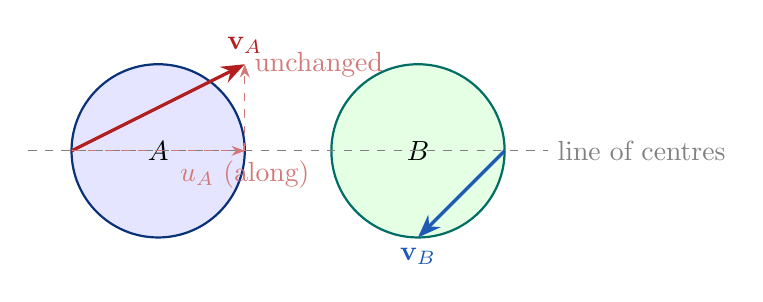
\begin{tikzpicture}[>=Stealth, scale=1.1]
  % Two spheres
  \draw[thick, deepblue, fill=blue!10] (-1.5, 0) circle (1);
  \draw[thick, tealgreen, fill=green!10] (1.5, 0) circle (1);
  
  % Labels
  \node at (-1.5, 0) {$A$};
  \node at (1.5, 0) {$B$};
  
  % Line of centres
  \draw[dashed, gray] (-3, 0) -- (3, 0) node[right] {line of centres};
  
  % Velocity A
  \draw[->, very thick, warmred] (-2.5, 0) -- (-0.5, 1) node[above] {$\vvec_A$};
  
  % Velocity B
  \draw[->, very thick, midblue] (2.5, 0) -- (1.5, -1) node[below] {$\vvec_B$};
  
  % Components
  \draw[->, dashed, warmred!60] (-2.5,0) -- (-0.5, 0) node[below] {$u_A$ (along)};
  \draw[->, dashed, warmred!60] (-0.5, 0) -- (-0.5, 1) node[right] {unchanged};
\end{tikzpicture}
\end{center}

\begin{exmp}{Oblique Collision}{}
A smooth sphere $A$ of mass $2\kg$ moves with velocity $\begin{pmatrix}6 \\ 0\end{pmatrix}\ms$ and hits an identical stationary sphere $B$. At impact, the line of centres is at $30^\circ$ to the direction of motion of $A$. $e = 0.8$. Find the velocities after impact.

\medskip
\textbf{Coordinates.} Let $x$ be along the line of centres ($30^\circ$ to original direction), $y$ perpendicular.

\textbf{Resolve $A$'s initial velocity along these axes:}
\[
  u_{Ax} = 6\cos 30^\circ = 3\sqrt{3}\ms, \quad u_{Ay} = 6\sin(-30^\circ) = -3\ms
\]
($B$ is stationary: $u_{Bx} = u_{By} = 0$.)

Wait --- actually the line of centres is at $30^\circ$ to $A$'s motion direction. Let's say $A$ moves in the $X$ direction and the line of centres makes $30^\circ$ with $X$. Resolving $A$'s velocity:

Along line of centres: $u_{Ax} = 6\cos 30^\circ = 3\sqrt{3}$

Perpendicular: $u_{Ay} = -6\sin 30^\circ = -3$ (or $+3$ depending on geometry)

\textbf{Along line of centres (momentum + restitution):}

Momentum: $2u_{Ax} + 0 = 2v_{Ax} + 2v_{Bx} \implies v_{Ax} + v_{Bx} = 3\sqrt{3}$

Restitution: $v_{Bx} - v_{Ax} = e \cdot u_{Ax} = 0.8 \times 3\sqrt{3} = 2.4\sqrt{3}$

Adding: $2v_{Bx} = 3\sqrt{3} + 2.4\sqrt{3} = 5.4\sqrt{3} \implies v_{Bx} = 2.7\sqrt{3} \approx 4.68\ms$

$v_{Ax} = 3\sqrt{3} - 2.7\sqrt{3} = 0.3\sqrt{3} \approx 0.52\ms$

\textbf{Perpendicular to line of centres:} Velocities unchanged.

$v_{Ay} = u_{Ay} = -3\ms$ (or $+3\ms$ depending on sign convention)

$v_{By} = 0$ (B was stationary and no impulse acts perpendicularly)
\end{exmp}

\subsection{Collision with a Wall}

When a smooth ball hits a smooth wall, the wall exerts an impulsive force normal to the wall. The component of velocity along the wall is unchanged; the component normal to the wall is reversed and reduced by factor $e$.

\begin{exmp}{Ball Hitting a Smooth Wall}{}
A ball moving at $\begin{pmatrix} 4 \\ -3 \end{pmatrix}\ms$ hits a smooth vertical wall ($y$-axis). $e = 0.6$ for the wall. Find the velocity after impact.

\medskip
Wall is vertical; impulse acts horizontally (normal to wall).

Normal component (horizontal, $x$-direction): reversed and multiplied by $e$: $v_x = -(-4) \times 0.6$... Wait, carefully: the ball hits the wall moving to the left ($x$ component $= -4$? or right?).

Let the wall be at $x = 0$, ball moving in $+x$ direction. $u_x = 4$, $u_y = -3$.

After impact: $v_x = -eu_x = -0.6 \times 4 = -2.4\ms$ (bounces back)

$v_y = u_y = -3\ms$ (unchanged, along wall)

Speed after: $\sqrt{2.4^2 + 3^2} = \sqrt{5.76 + 9} = \sqrt{14.76} \approx 3.84\ms$
\end{exmp}

\section{Energy in Collisions}

\begin{thm}{Energy Lost in a Collision}{}
For two particles of equal mass $m$ with velocities $u_1, u_2$, coefficient of restitution $e$:
\[
  \Delta KE = \tfrac{1}{2}m(1-e^2)(u_1-u_2)^2 \cdot \frac{m_1m_2}{(m_1+m_2)^2}\cdot 2(m_1+m_2)
\]
More simply, for general masses:
\[
  \text{KE lost} = \tfrac{1}{2}\mu(1-e^2)(u_1-u_2)^2
\]
where $\mu = \frac{m_1m_2}{m_1+m_2}$ is the \textbf{reduced mass}.

For a perfectly elastic collision ($e=1$): no energy lost.
For a perfectly inelastic collision ($e=0$): maximum energy lost.
\end{thm}

\section{Advanced: Multiple Collisions}

\begin{exmp}{Three Particles in a Line}{}
Three identical particles $A$, $B$, $C$ (each mass $m$, $e = 0.5$) lie in a line. $A$ moves at $u$ toward $B$ and $C$ (at rest). Describe all subsequent collisions.

\medskip
\textbf{First collision ($A$ hits $B$):}

Momentum: $mu = mv_A + mv_B \implies u = v_A + v_B$

Restitution: $v_B - v_A = 0.5u$

$\implies v_B = \frac{3u}{4}$, $v_A = \frac{u}{4}$

\textbf{Second collision ($B$ hits $C$):}

Similarly: $v_C = \frac{3}{4}v_B = \frac{9u}{16}$, $v_B' = \frac{1}{4}v_B = \frac{3u}{16}$

\textbf{Does $A$ catch $B$?} $A$ moves at $\frac{u}{4}$, $B$ now moves at $\frac{3u}{16} < \frac{u}{4}$, so $A$ \emph{is} faster than $B$: yes, $A$ will hit $B$ again.

This cascading behaviour is the basis for Newton's cradle and many important problems in collision dynamics.
\end{exmp}

\section{Connections and Advanced Ideas}

\begin{explorationbox}
\textbf{Elastic Collisions and Centre of Mass Frame.}
In the centre of mass (CM) frame (the frame moving with the total momentum of the system), the total momentum is zero. In a perfectly elastic collision in this frame, the speeds of the particles are unchanged but their directions reverse. Transforming back to the lab frame gives the velocities after collision. This technique is powerful in particle physics.
\end{explorationbox}

\begin{explorationbox}
\textbf{Noether's Theorem.}
The conservation of momentum is a direct consequence of the fact that the laws of physics are the same at every point in space (spatial translation symmetry). Emmy Noether proved in 1915 that every continuous symmetry of a physical system implies a conservation law. This is one of the most profound theorems in all of physics:
\[
\text{Translation symmetry} \leftrightarrow \text{Conservation of momentum}
\]
\[
\text{Time-translation symmetry} \leftrightarrow \text{Conservation of energy}
\]
\[
\text{Rotation symmetry} \leftrightarrow \text{Conservation of angular momentum}
\]
\end{explorationbox}

\begin{summarybox}[Chapter 18 Summary: Momentum]
\begin{itemize}[leftmargin=1.5em]
  \item Momentum: $p = mv$; vector quantity; units $\mathrm{kg\,m\,s}^{-1}$
  \item Newton's 2nd Law: $F = dp/dt$; impulse $J = \Delta p = F\Delta t$
  \item Conservation of momentum: $\sum m_i v_i = $ const (isolated system)
  \item Coefficient of restitution: $e = \frac{\text{speed of separation}}{\text{speed of approach}}$; $0 \leq e \leq 1$
  \item Direct collision: use momentum conservation + Newton's law of restitution
  \item Oblique collision: decompose into line-of-centres (apply restitution) and perpendicular (unchanged)
  \item Energy lost $= \frac{1}{2}\mu(1-e^2)(\text{speed of approach})^2$
  \item $e=1$: elastic (no energy loss); $e=0$: perfectly inelastic (coalesce)
\end{itemize}
\end{summarybox}

% =====================================================================
%  BACKMATTER
% =====================================================================
\backmatter

\chapter*{Formula Sheet}
\addcontentsline{toc}{chapter}{Formula Sheet}

\begin{summarybox}[Further Mechanics: Key Formulae]

\textbf{Chapter 13 --- Projectiles}
\begin{align*}
  x &= ut\cos\alpha & y &= ut\sin\alpha - \tfrac{1}{2}gt^2 \\
  T &= \tfrac{2u\sin\alpha}{g} & R &= \tfrac{u^2\sin 2\alpha}{g} \\
  H &= \tfrac{u^2\sin^2\alpha}{2g} & \text{Traj.}: y &= x\tan\alpha - \tfrac{gx^2\sec^2\alpha}{2u^2}
\end{align*}

\textbf{Chapter 14 --- Equilibrium}
\begin{align*}
  M &= Fd & \bar{x} &= \tfrac{\sum m_ix_i}{\sum m_i} \\
  \bar{x}_{\text{cone}} &= \tfrac{h}{4} \text{ from base} & \bar{x}_{\text{hemi}} &= \tfrac{3r}{8} \text{ from flat face}
\end{align*}

\textbf{Chapter 15 --- Circular Motion}
\begin{align*}
  v &= r\omega & a &= \tfrac{v^2}{r} = r\omega^2 \\
  F &= \tfrac{mv^2}{r} & T_{\text{period}} &= \tfrac{2\pi}{\omega} \\
  v_{\min}^{\text{top}} &= \sqrt{gr} & v_{\min}^{\text{bottom}} &= \sqrt{5gr}
\end{align*}

\textbf{Chapter 16 --- Hooke's Law}
\begin{align*}
  T &= \tfrac{\lambda x}{l_0} = kx & E_{\text{EPE}} &= \tfrac{\lambda x^2}{2l_0} = \tfrac{1}{2}kx^2
\end{align*}

\textbf{Chapter 17 --- Variable Force}
\begin{align*}
  a &= v\tfrac{dv}{dx} & \tfrac{1}{2}mv^2 &= \int F\,dx + C \\
  v_T &= \sqrt{mg/k} \text{ (terminal)} & &
\end{align*}

\textbf{Chapter 18 --- Momentum}
\begin{align*}
  J &= \Delta p = F\Delta t & p &= mv \\
  e &= \tfrac{v_B'-v_A'}{u_A-u_B} & \Delta KE &= \tfrac{1}{2}\mu(1-e^2)(\Delta u)^2
\end{align*}

\end{summarybox}

\chapter*{Extension Problems}
\addcontentsline{toc}{chapter}{Extension Problems}

\begin{explorationbox}[Challenge Problems]
\begin{enumerate}[leftmargin=1.5em, label=\textbf{E\arabic*.}]
  \item \textbf{(Projectiles)} A particle is projected from a point $O$ with speed $u$ at angle $\alpha$ above a plane inclined at $\beta$ to the horizontal. Derive the range along the inclined plane and show that the maximum range along the plane is $\frac{u^2}{g(1+\sin\beta)}$.
  
  \item \textbf{(Equilibrium)} A uniform solid hemisphere of radius $r$ and mass $m$ rests with its curved surface on a rough inclined plane (angle $\theta$). Show that the hemisphere does not slip if $\mu \geq \frac{3}{8}\tan\theta$ and find the condition for it not to topple.
  
  \item \textbf{(Circular Motion)} A bead of mass $m$ slides on a smooth circular wire of radius $r$ fixed in a vertical plane. The bead starts from rest at the top. Find the normal reaction as a function of angle, and show that it first becomes zero at $\cos\theta = 2/3$ from the vertical.
  
  \item \textbf{(Hooke's Law)} Two identical springs, each of natural length $l_0$ and modulus $\lambda$, are connected in series and in parallel. Show that the effective spring constants are $k/2$ and $2k$ respectively, where $k = \lambda/l_0$.
  
  \item \textbf{(Variable Force)} A particle of mass $m$ moves in a medium where the resistance force is $F_R = -mkv$ for low speeds and $F_R = -mk^2v^2$ for high speeds. At what speed does the transition occur and what is the terminal velocity in each regime?
  
  \item \textbf{(Momentum)} Three identical balls in a line, coefficient of restitution $e$, are set in motion: show that after all collisions are complete, the final speeds form a geometric sequence and find the common ratio.
  
  \item \textbf{(University Level)} Using the work-energy theorem, prove that for a conservative force $\Fvec = -\nabla V$ (gradient of potential energy $V$), the total mechanical energy $E = \frac{1}{2}mv^2 + V$ is conserved. How does this connect Hooke's Law (EPE), gravity (GPE), and all conservative forces?
\end{enumerate}
\end{explorationbox}

\end{document}